\section{Planet detection statistics}  
\label{sec:newly_detected_planet_metrics}

Using the planet detection model described in Sec.~\ref{sec:planet_detection_model} and the target selection procedure of Sec.~\ref{sec:selection_criteria}, we simulate three years of \tess observing, with for six different possibilities for the third year:
\nhemi, \npole, \shemiAvoid, \elong, \eshort, and \hemis.
How many new planets do we detect, and how do their properties differ between extended missions?

\subsection{Planet Yield from the Primary Mission}
\label{sec:results_from_primary_missions}
\begin{marginfigure} %[t]
	\centering
	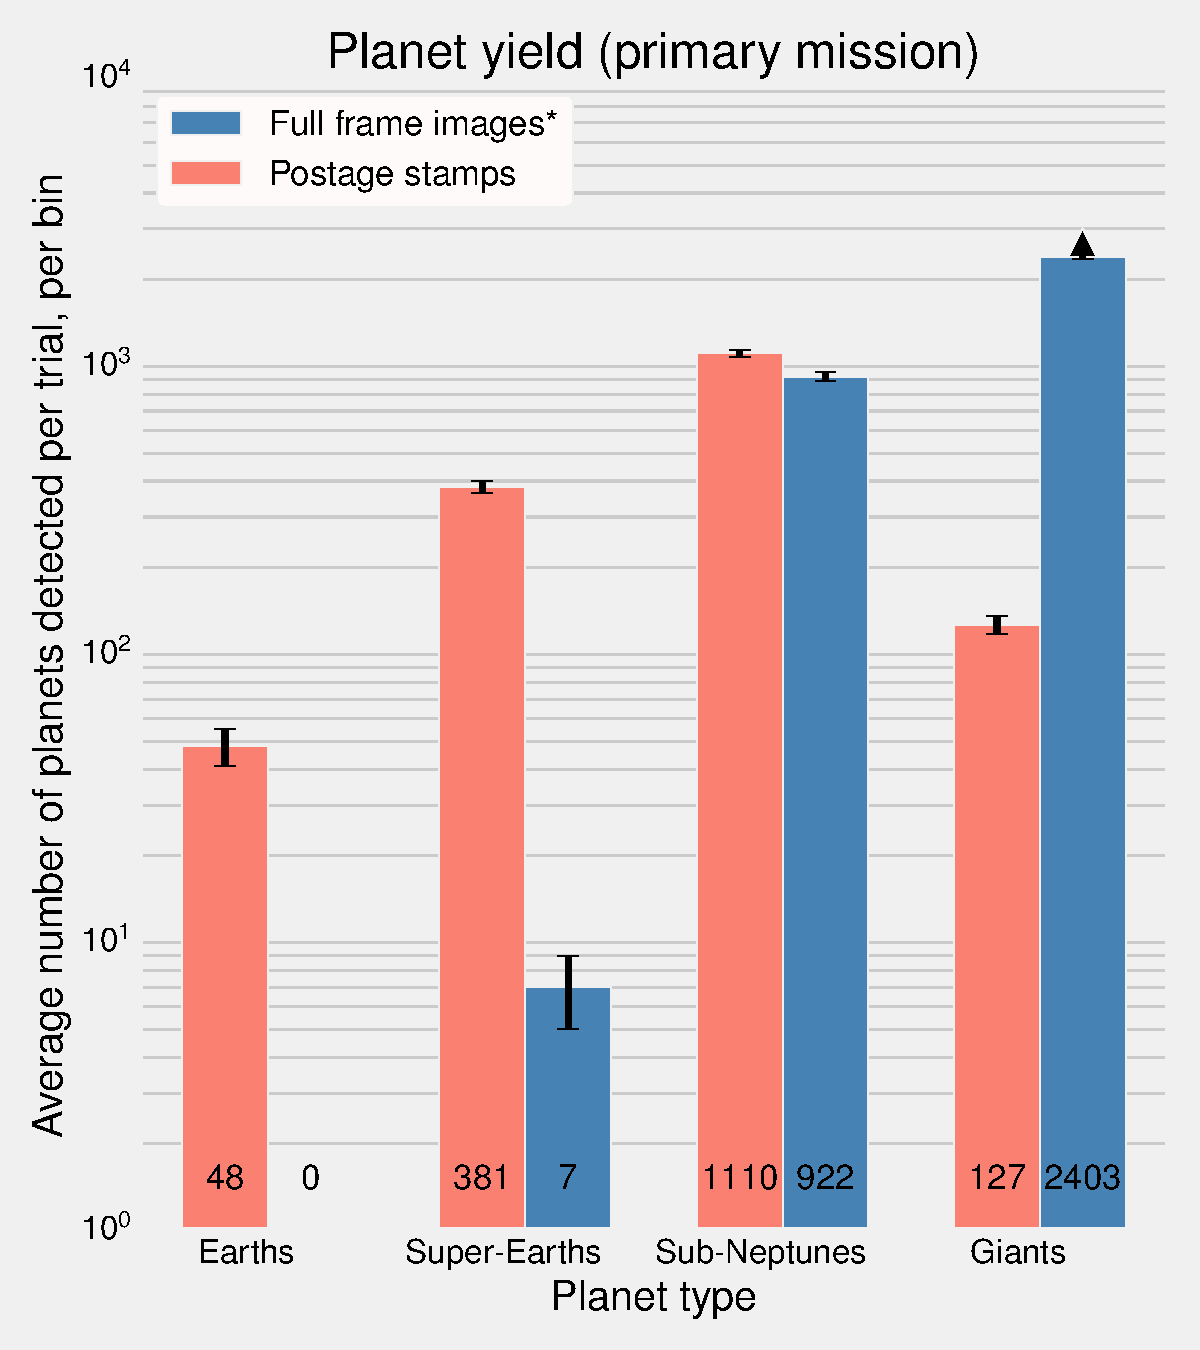
\includegraphics[width=\textwidth]{figures/160729_pm0_shemi_nhemi_nhemi_t20-pri-yield.pdf}
	\caption{Mean numbers of planets detected in \tesss Primary Mission.
	The number of Earths ($R_p < 1.25R_\oplus$), super-Earths ($1.25R_\oplus \le R_p < 2R_\oplus$), sub-Neptunes ($2R_\oplus \le R_p < 4R_\oplus$) and giants agree with the respective values quoted in \protect\citet{Sullivan_2015} to $\lesssim 50\%$. 
	%despite modifications to our target selection procedure (Sec.~\protect\ref{sec:selection_criteria}).
	Our full frame images detections are complete for $R_p < 4R_\oplus$, and 
	incomplete for giant ($R_p > 4R_\oplus$) planets, shown with a lower limit 
	(see text for discussion). 
	Error bars are from only Poisson fluctuations and do not account for systematic uncertainty.}
	\label{fig:primary_planet_yield}
\end{marginfigure}
We first examine our results for just the Primary Mission -- the first two years of \tesss observing. 
We follow with an analysis of our detected planet populations from a single Year-3 Extended Mission (Sec.~\ref{sec:results_from_nhemi_extended_mission}), and then all six of our proposed Extended Missions (Sec.~\ref{sec:results_from_all_extended_missions}).
Here we highlight commonalities and differences between~\citetalias{Sullivan_2015} and this work.

\paragraph{Detected planet yield}
The first point of consideration is the detected planet yield, shown in Fig.~\ref{fig:primary_planet_yield}.
The number of Earths, super-Earths, and sub-Neptunes we detect agrees with the 
numbers quoted by~\citetalias{Sullivan_2015} to within $50\%$, despite the 
modifications described in Sec.~\ref{sec:selection_criteria} to the target 
selection procedure.
Other changes to our simulation's assumptions, for instance using an as-built 
model of \tesss PSF informed by laboratory tests (courtesy Deborah Woods) 
rather than the idealized PSF described in Sec 6.1 
of~\citetalias{Sullivan_2015}, had only minor impact on this final result 
($10\%$ change in yield).

A modification that did influence our lowered expected yields was a bug-fix 
from~\citetalias{Sullivan_2015}'s dilution calculation. Recall our definition 
of 
the dilution parameter $D$ (Eq.~\ref{eq:dilution}): placing a binary companion 
with luminosity identical to the host star into a system with a transiting 
planet that would typically transit with depth $\delta$ leads to a transit with 
`effective depth' $\delta/2$. A single missing symbol\footnote{An $\texttt{=}$ rather than 
a $\texttt{+=}$} led~\citetalias{Sullivan_2015} to under-account for this 
effect, which 
in our simulations brought about factors of $1.5\times, 1.3\times,\ 
\mathrm{and}\ 1.2\times$ fewer Earths, super-Earths, and sub-Neptunes 
respectively. This error can be noted in Table 6 
of~\citetalias{Sullivan_2015}, where nearly all the dilution parameter 
values are near 1.


An additional note is that in the preparation of this report, a glaring 
discrepancy emerged between our predicted $\approx 400$ super-Earth detections 
and those shown in Fig.~18 of~\citetalias{Sullivan_2015}, which 
displays $\approx 1400$ planets. The subsequent investigation led to the 
discovery of a bug in the plotting script used to create 
Fig.~18~\citetalias{Sullivan_2015} (erratum in preparation). The 
error did not
affect any of the results described in~\citetalias{Sullivan_2015}'s text, or 
the simulation results that were tabulated in the paper and sent electronically 
to interested parties.
The corrected version 
of~\citetalias{Sullivan_2015}'s Fig. 18 shows $\approx 500$ expected 
super-Earths, which closely agrees with our work when also accounting for the 
dilution error described above.


\begin{comment}
However, our yields from full frame images differ markedly from those quoted in Fig. 18 of~\citetalias{Sullivan_2015}.
We agree with~\citetalias{Sullivan_2015} that no Earths are detected in the full frame images.
However, we detect only $\sim$10 super-Earths by observing the $200,001\mathrm{^{st}}$ to $4,000,000\mathrm{^{th}}$ \texttt{Merit}-ranked stars at 30 minute cadence.
This is two orders of magnitude less than the $\sim$1000 super-Earth detections claimed from FFIs by~\citetalias{Sullivan_2015}.
There is also a discrepancy in FFI-detected sub-Neptunes, for which our current simulations predict that $\sim$1000 will be detected,
while~\citetalias{Sullivan_2015} predicted $\sim$2000.

We empirically verified that our full frame image detections are complete for $R < 4R_\oplus$ by enlarging the number of stars observed at 30-minute cadence and seeing that the number of detected planets with radii less than Neptune did not change.
%In this context,~\citetalias{Sullivan_2015}'s claim of detecting $1000$ super-Earths in \tesss full-frame images must be false.
We do not understand the origin of the difference between our method and~\citetalias{Sullivan_2015}'s, even after corresponding with P. Sullivan, but note that our results are in much better agreement with order-of-magnitude analytic arguments for \tesss expected planet yield.
Assuming an exponentially distributed stellar population in the galaxy and computing limiting magnitude thresholds,~\citet{winn_searchable_2013} predicted detections of $600-6000$ Neptunes, $24-300$ super-Earths, and $1-10$ Earth-sized planets, where the lower bounds correspond to planets detected with $\mathrm{SNR}>10$, and the upper bounds $\mathrm{SNR}>7$.
~\citetalias{Sullivan_2015}'s prediction of a total of $1500$ detected super-Earths is a factor of 5 larger than these analytic estimates, while
ours is in much better agreement.

Another plausibility argument that our current treatment of the FFIs
is delivering more accurate results than the code employed
by~\citetalias{Sullivan_2015} is that starting from the same input
distribution of planets, we find a more reasonable detection bias
against small planets.
One should expect that the detection bias against small planets is a steep function of radius, given that $\delta\propto R_p^2$.
\citetalias{Sullivan_2015} predicted the detection of roughly twice as many sub-Neptunes as super-Earths; our current
result has the ratio is closer to 5-to-1 which seems more realistic.
\end{comment}


\begin{comment}
  Consider the two relevant bins in the
  distribution of detected planet count \textit{vs}. planet radius.
  The $1.25R_\oplus<R_p<2R_\oplus$ bin has width $0.75R_\oplus$ and
  contains 1400 (400) detected planets according
  to~\citetalias{Sullivan_2015} (according to us).  The
  $2R_\oplus<R_p<4R_\oplus$ bin has width $2R_\oplus$ and contains 3000 (2000)
  detected planets according to~\citetalias{Sullivan_2015}
  (according to us).  The ratio of the number of detected super-Earths
  to sub-Neptunes, adjusted to the same bin width $\Delta R_p=0.75~R_\oplus$,
  is $(1400/0.75R_\oplus)/(3000/2R_\oplus)=1.25$ for \citetalias{Sullivan_2015}
  and $(400/0.75R_\oplus)/(2000/2R_\oplus)=0.53$ for our current simulations.

  The input planet occurrence distributions
  (\citetalias{Sullivan_2015}'s Fig 8) imply that the intrinsic
  population ratio in this bin is $\sim\!2$ for $T_\mathrm{eff}<4000$K
  hosts and $\sim\!1.5$ for $T_\mathrm{eff}>4000$K hosts.  Thus the
  input ratio for the number of existing super-Earths (per bin width)
  to sub-Neptunes (per bin width) across all stars is between 1.5 and
  2.
\end{comment}

% Also, Peter's data from plat10r.fits, May 4 2015, agree with my results. I never was able to find the data with his FFI numbers...

\paragraph{Properties of planets detected in Primary Mission} 

We show the population properties of planets detected in postage
stamps and full frame images during the Primary Mission in
Figs.~\ref{fig:radius_vs_period_nhemi}
and~\ref{fig:imag_vs_teff_nhemi}.  In terms of the apparent planet
radii $R_p$, orbital periods $P$, host star brightness, and host star
$T_\mathrm{eff}$, we qualitatively agree with the results
of~\citetalias{Sullivan_2015} for the planets detected
in postage stamps. 
For instance, the dearth of $P<5$ day
Neptune-radius ($R_p \lesssim 4R_\oplus$) planets in 
Fig.~\ref{fig:radius_vs_period_nhemi} was
observed by \textit{Kepler}~\citep{mazeh_dearth_2016}, and thus it is
present in our input occurrence rates, rather than being an
observational bias.  It was also seen by~\citetalias{Sullivan_2015}.

The differences between planets detected in postage stamps vs. in full frame images follow our expectation from our \texttt{Merit} statistic. 
Namely, Fig.~\ref{fig:imag_vs_teff_nhemi} shows that at a fixed brightness, full frame image detections tend to occur at larger stellar effective temperature (and thus stellar radius).
At a fixed host star radius, postage stamp detections occur around brighter stars.

\paragraph{Impact of earth and moon crossings on Primary Mission's detected planet yield}
During the Primary Mission, of the four cameras, Camera 1 (closest to the 
ecliptic) suffers the most from Earth and Moon crossings.
As noted in Table~\ref{tab:dropped_fields}, we remove 4 of its 13 
`observing sectors' from that year.
This reduces the number of planet detections near the ecliptic, and is visible in the orange points of Fig.~\ref{fig:skymap_nhemi}.
In the Primary Mission \tess detects $\sim20$ planets with $R_p<4R_\oplus$ 
(PS+FFI) in each $24^\circ\times24^\circ$ camera field nearest to the ecliptic.
As implemented in our simulation, Earth and Moon crossings result in some 
fields simply not being observed, so in these cases planets orbiting stars in 
these fields are never detected.
Considering only the Primary Mission, we would naively expect that dropping a total of 9 fields over the two years (again, see Table~\ref{tab:dropped_fields}) would result in a loss of $\sim9\times20=180$ planets.
This agrees with what our simulations actually give: running them without accounting for Earth and Moon losses returns a mean of 2678 detected planets with $R_p<4R_\oplus$, while running them with Earth and Moon crossings gives a mean of 2482 such planets (a loss of 196 planets; $7\%$ of the $R_p<4R_\oplus$ planet yield).
% data from 160708-t50 and 160729-t20. Slightly apples to oranges because of number of trials difference, but makes the point. 


\subsection{Planet yield from an example Extended Mission (\rm{\nhemi}) }
\label{sec:results_from_nhemi_extended_mission}

\begin{figure*}[t]
	\centering
	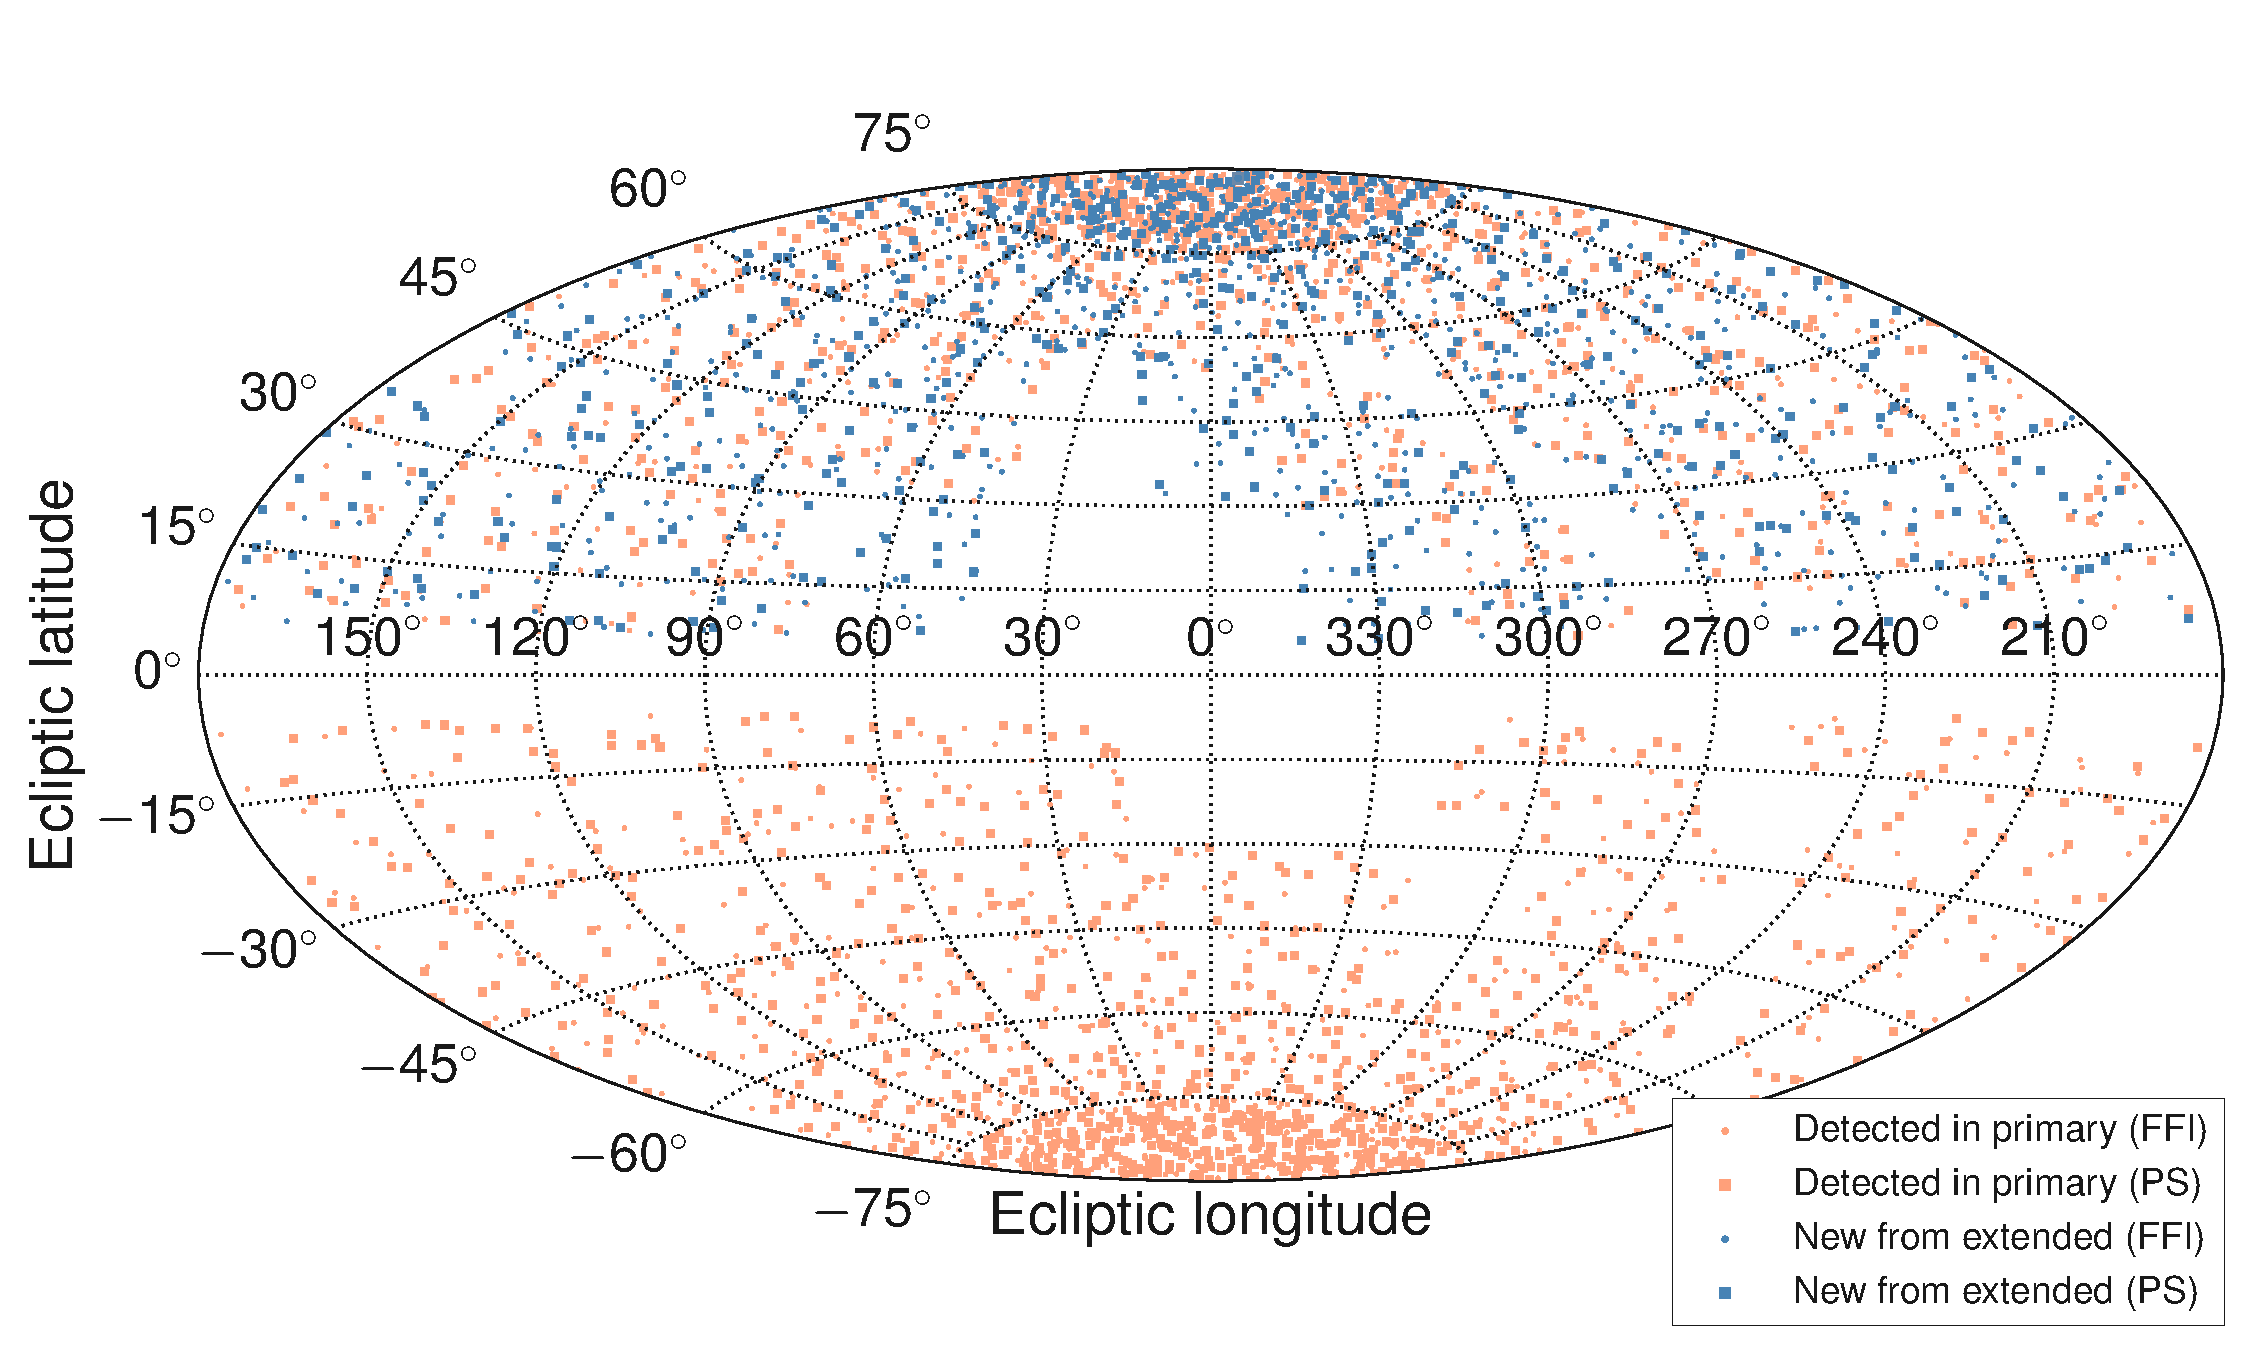
\includegraphics[]{figures/skymap_dropped_fields.pdf}
	\caption{Positions of $R_p<4R_\oplus$ planets detected in the \npole\:scenario. Squares (postage stamps) and dots (full frame images) are observed at 2 and 30 minute cadence respectively. Orange denotes detection over the first two years of observing (the Primary Mission), and blue denotes newly detected planets from the extra third year. The `gaps' in fields due to Earth and Moon crossings during the primary and Extended Missions are noted in Table~\protect\ref{tab:dropped_fields}. For instance, the field centered at $(\lambda=330^\circ,\beta=18^\circ)$ is observed in the extended but not the Primary Mission. }
	\label{fig:skymap_nhemi}
\end{figure*}
\begin{figure*}[t]
	\centering
	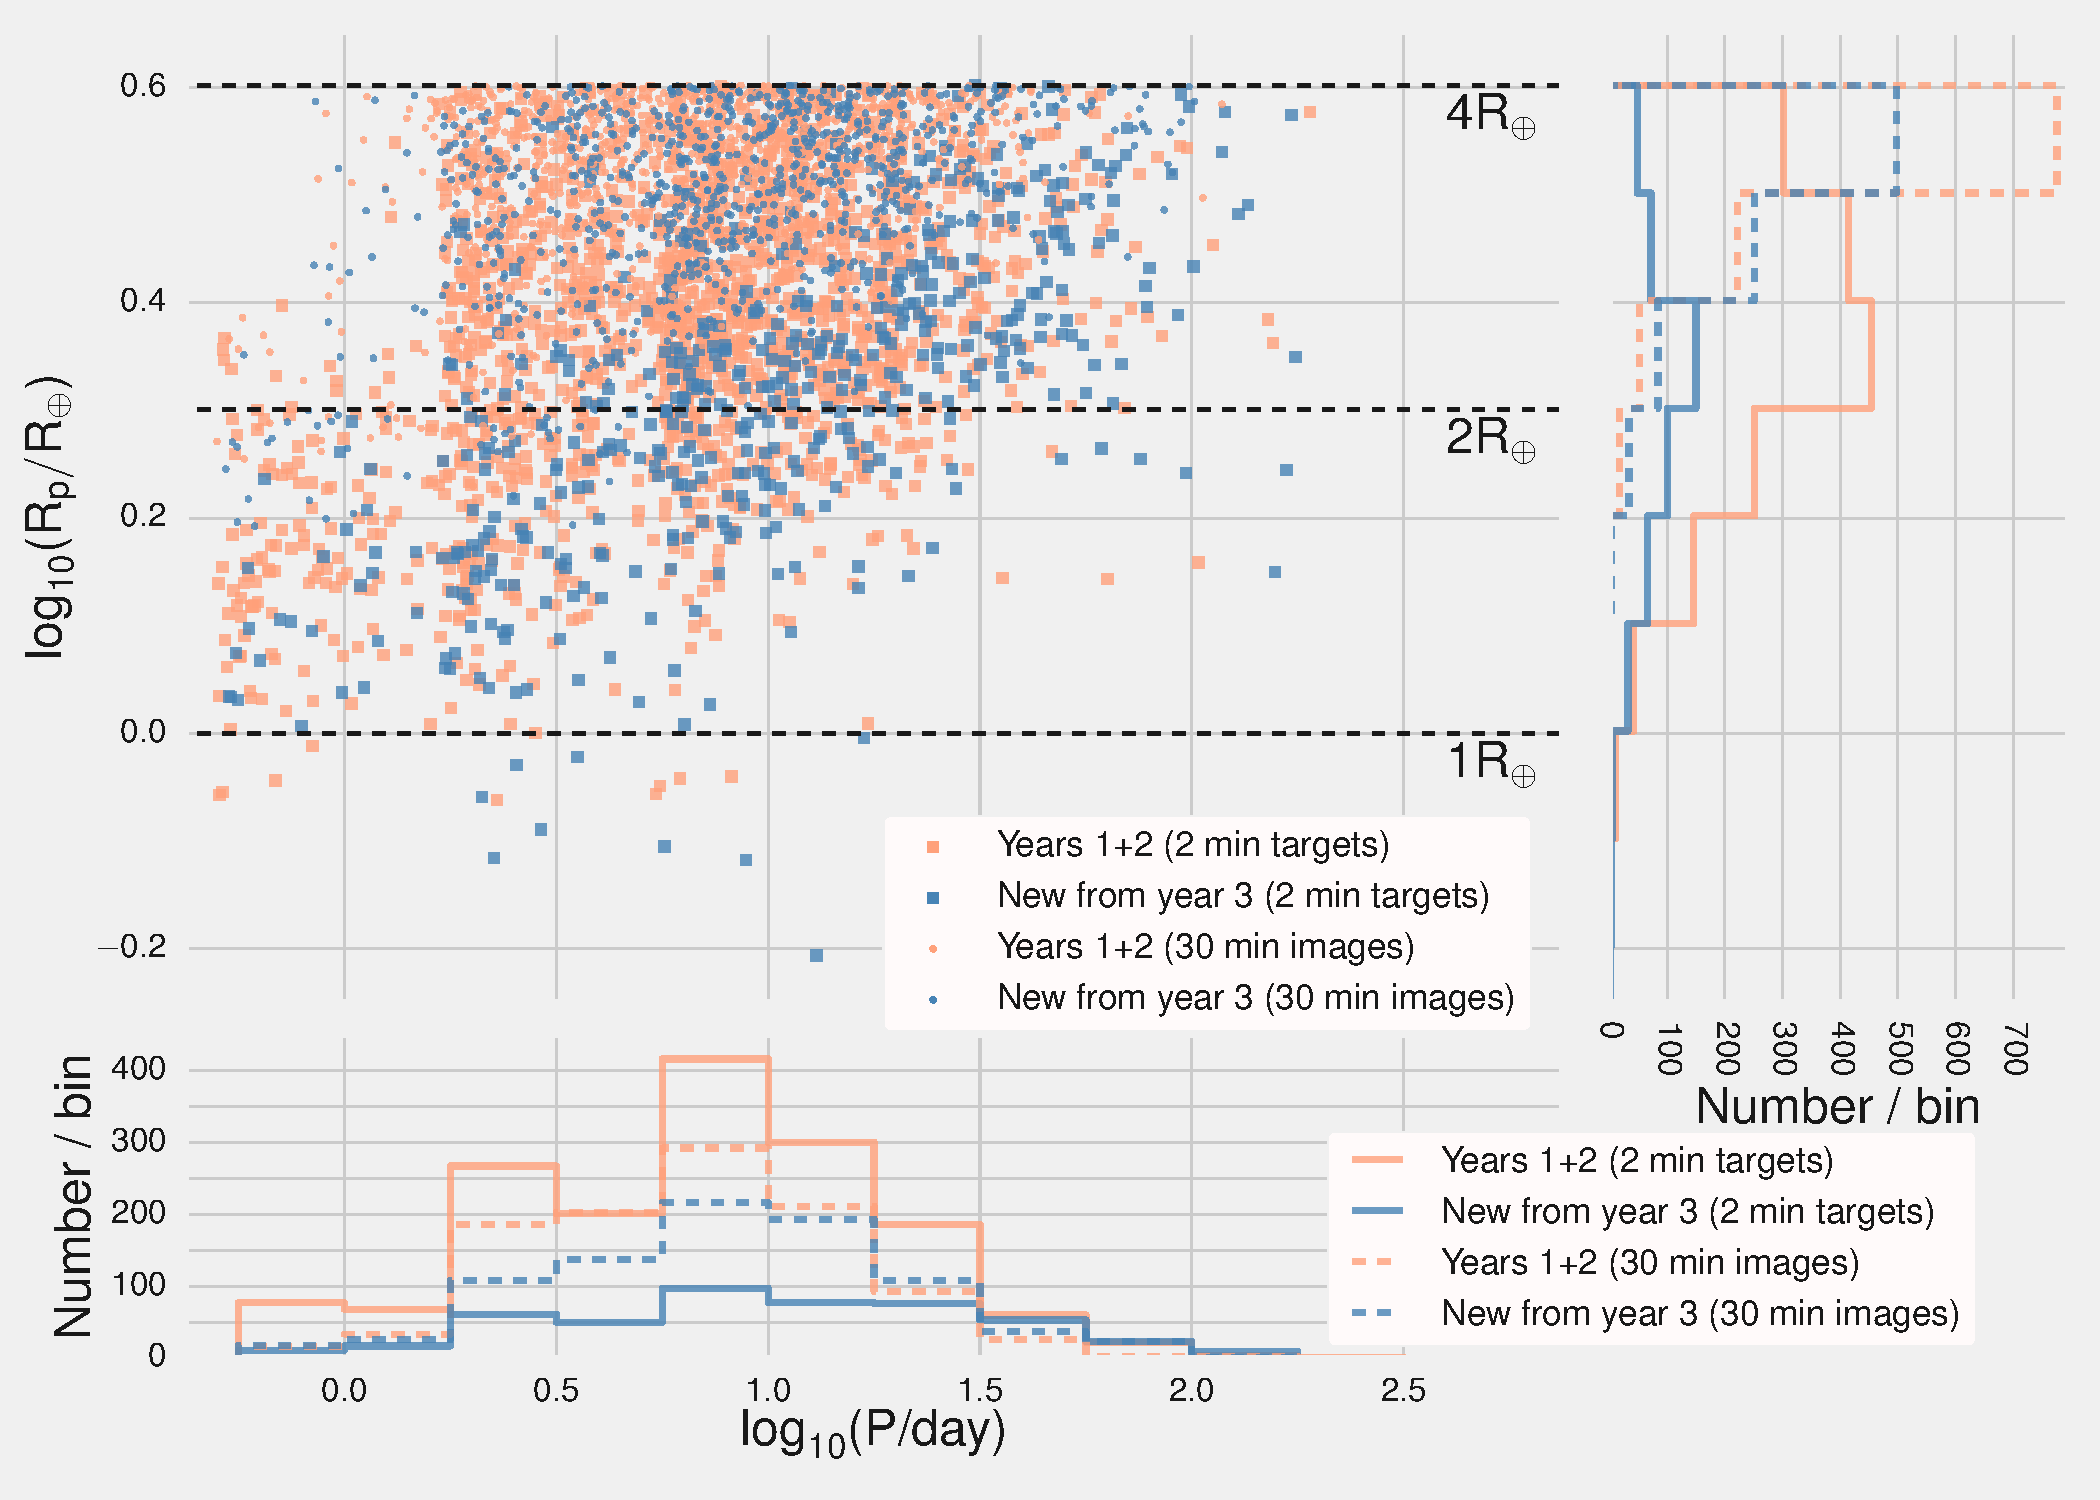
\includegraphics[]{figures/logR_vs_logP.pdf}
	\caption{Radius vs period of detected $R_p<4R_\oplus$ planets from one Monte Carlo realization of the \npole\:scenario.
	At a fixed period, Extended Missions help us detect smaller planets; at a fixed radius, they let us probe out to longer periods.
	The radius histogram, and the location of all dots (rather than squares) on the scatter plot show that almost all $R_p<2R_\oplus$ planets are detected in postage stamps, not full frame images (also shown in Fig.~\protect\ref{fig:primary_planet_yield}).}
	\label{fig:radius_vs_period_nhemi}
\end{figure*}
\begin{figure*}[t]
	\centering
	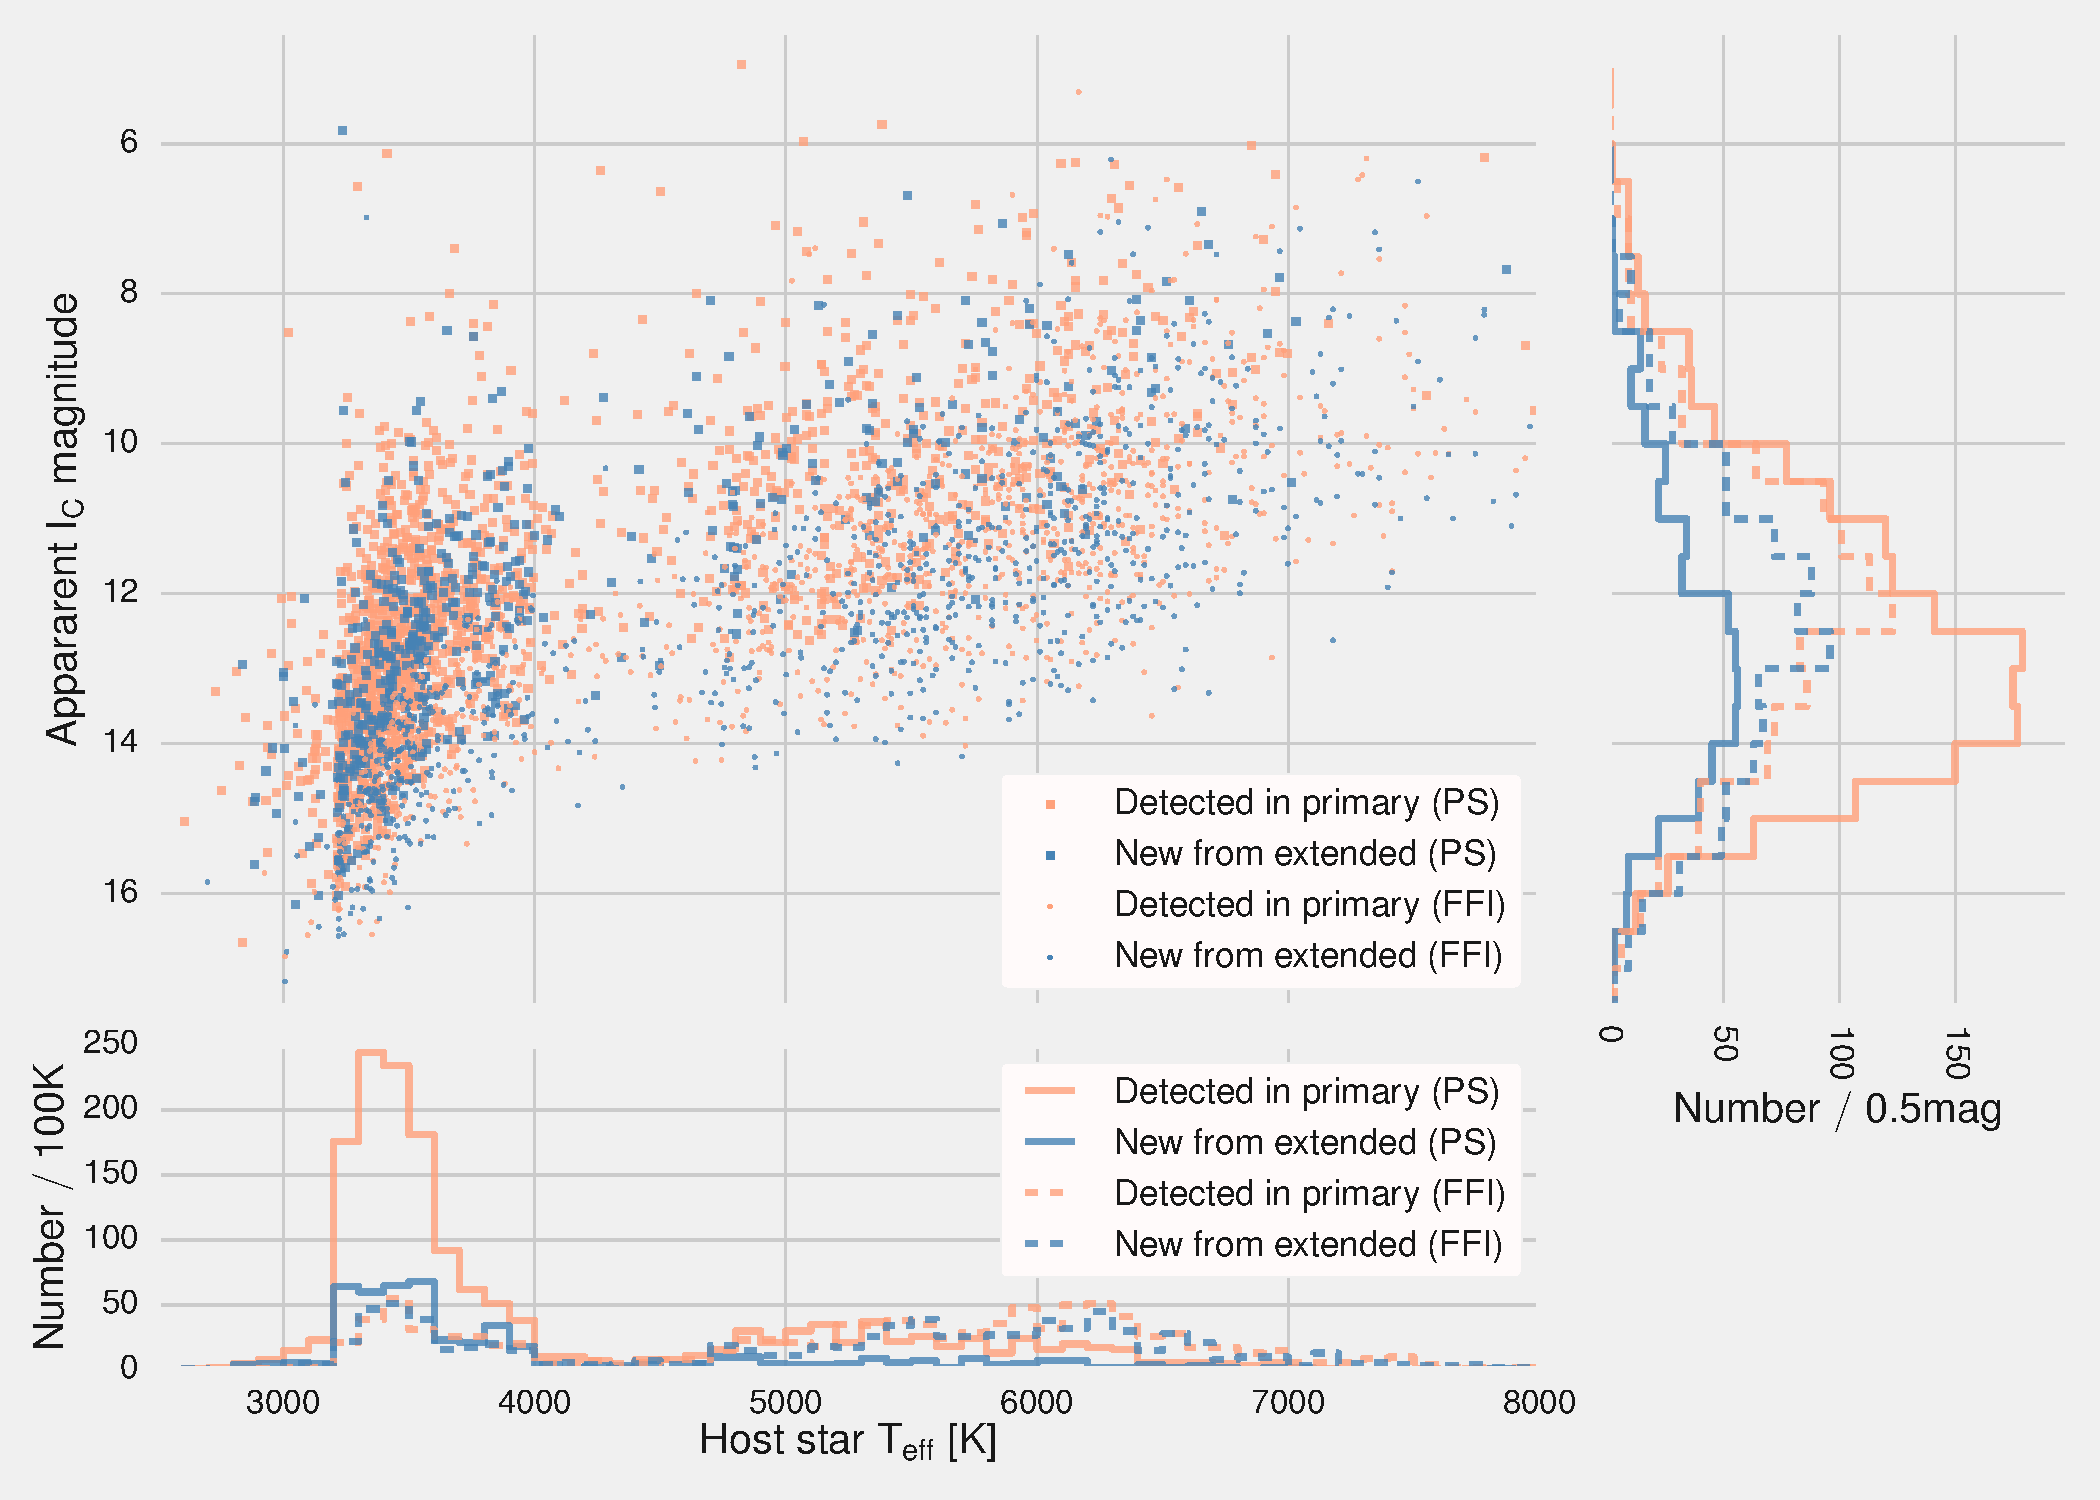
\includegraphics[]{figures/temp_imag_vs_teff_nhemi.pdf}
	\caption{Apparent Cousins I magnitude plotted against effective temperature for $R_p<4R_\oplus$ planets detected from one Monte Carlo realization of the \npole\:scenario. 
	Postage stamp (PS) detections are biased towards M dwarfs in part because of our selection procedure.
	For a given effective temperature, full frame images (FFIs) are taken of dimmer stars.}
	\label{fig:imag_vs_teff_nhemi}
\end{figure*}
	%all from 160729 runs. In this case for nhemi.

Before comparing our six selected Extended Mission scenarios simultaneously (Sec.~\ref{sec:results_from_all_extended_missions}), we describe the detected planet populations from a single realization of an Extended Mission.
As an example case, we choose the \npole\:scenario.

A sky map showing the positions of detected planets for this mission is drawn in Fig.~\ref{fig:skymap_nhemi}.
Commenting on this map, we note that:
\begin{itemize}
	\item Any planet detected in this scenario's Primary Mission is also detected in its Extended Mission.
	We consequently color the detected planets depending on if they are discovered in the Primary Mission, or whether they are detected only by virtue of the extra data collected in the Extended Mission.
	In our simulation, these extra observations will lead to new detections (a) because of an increased number of observed transits leading to a higher phase-folded SNR, which causes the transiting object's SNR to clear our threshold of 7.3, and/or (b) because raising the number of observed transits clears the minimum number of transits we require for detections ($N_\mathrm{tra} \geq 2$).
	\item The `dropped' fields described in Sec.~\ref{sec:earth_moon_crossings} owing to Earth/Moon crossings are visible for both the primary and Extended Missions in the $\lambda=(30^\circ, 0^\circ, 330^\circ, 300^\circ)$ fields.
\end{itemize}

In addition to examining the positions of the detected planets, we select and plot some of their key properties:
planet radius $R_p$, orbital period $P$, apparent magnitude $I_c$, and effective temperature $T_\mathrm{eff}$.
See Figs.~\ref{fig:radius_vs_period_nhemi} and~\ref{fig:imag_vs_teff_nhemi}.
Both of these figures are visualizations from a single Monte Carlo realization of the \npole\:scenario, and only show planets with $R_p < 4R_\oplus$.
These plots clarify a few points:
\begin{itemize}
	\item At a fixed period, Extended Missions help us detect smaller planets; at a fixed radius, they let us probe out to longer periods. This is one of the major reasons to extend \tesss observations.
	\item Almost all $R_p<2R_\oplus$ planets are detected in postage stamps, not full frame images. This is an indication that the top $2\times10^5$ \texttt{Merit} stars are a sufficient sample to detect most of the $R_p<2R_\oplus$ planets that \tess can detect.
	\item Postage stamp detections are biased towards M dwarfs. Per Fig.~\ref{fig:fig17_replica}, this is largely because our selection procedure chooses many M dwarfs.
	\item For a given effective temperature, full frame images detect planets about dimmer stars. Projecting the FFI detections onto apparent $I_c$ magnitude (Fig.~\ref{fig:imag_vs_teff_nhemi}, right panel), the median brightness of stars with planets detected from FFIs is actually greater than the median brightness of planets detected from PSs. This is because these detections are about stars with radii that, on average, are greater than those from postage-stamp detections.
	%\item The large number of full frame image detections between $5000\mathrm{K} < T_\mathrm{eff} < 7000\mathrm{K}$ suggest that our proposed selection procedure (Sec.~\protect\ref{sec:selection_criteria}) may not be optimal, and that a robust approach towards target prioritization, for instance using expected planet occurrence rates as a function of stellar type in a Bayesian approach, could maximize \tesss expected yield. 
\end{itemize}

There are a few other statistics that interesting for purposes of characterizing the value of this Extended Mission -- how many new planets do we detect? How many are at long orbital periods? How many are in habitable zones? We respond to these questions in Sec.~\ref{sec:results_from_all_extended_missions}, in particular showing our detected planet yields in Fig.~\ref{fig:yield_results}.


\subsection{Comparing Planet Yields from all Extended Missions}
\label{sec:results_from_all_extended_missions}
To compare Extended Missions in terms of planet detection statistics, we focus on the subset of all detected planets that are \textit{newly} detected from each Extended Mission.
These may come from stars that were not observed at all in the Primary Mission (notably for scenarios such as \elong), or they may also come from transiting planets that were observed in the Primary Mission with $\mathrm{SNR}<7.3$, or from planets that were single-transiters in the Primary Mission (we require $N_\mathrm{tra}\geq2$) for detection.
With this in mind, for each Extended Mission scenario we ask the following questions:

\begin{enumerate}
	\item $N_\mathrm{new}$: How many new planets do we detect?
	\item $N_\mathrm{new,P>20d}$: How many of these new planets are at long orbital periods, for instance $P>20$ days?
	\item $N_\mathrm{new,HZ}$: How many are in the habitable zone?
	\item $N_\mathrm{sys,extra\ planets}$: In how many systems in which at least one planet was detected during the Primary Mission do we find extra planets in the Extended Mission?
	\item $N_\mathrm{new,atm}$: How many new planets do we find that are amenable to atmospheric characterization (defined below by Eq.~\ref{eq:atmosphere_Deming})?
	\item $N_\mathrm{new,new\ stars}$: How many of the new planets come from 
	stars that were not observed in the Primary Mission? 
	\item $N_\mathrm{new,SNR\lor N_{tra}}$ stars that were observed, but either did not have enough transits or a high enough SNR to result in a detection?
\end{enumerate}
\begin{figure}[!t]
	\centering
	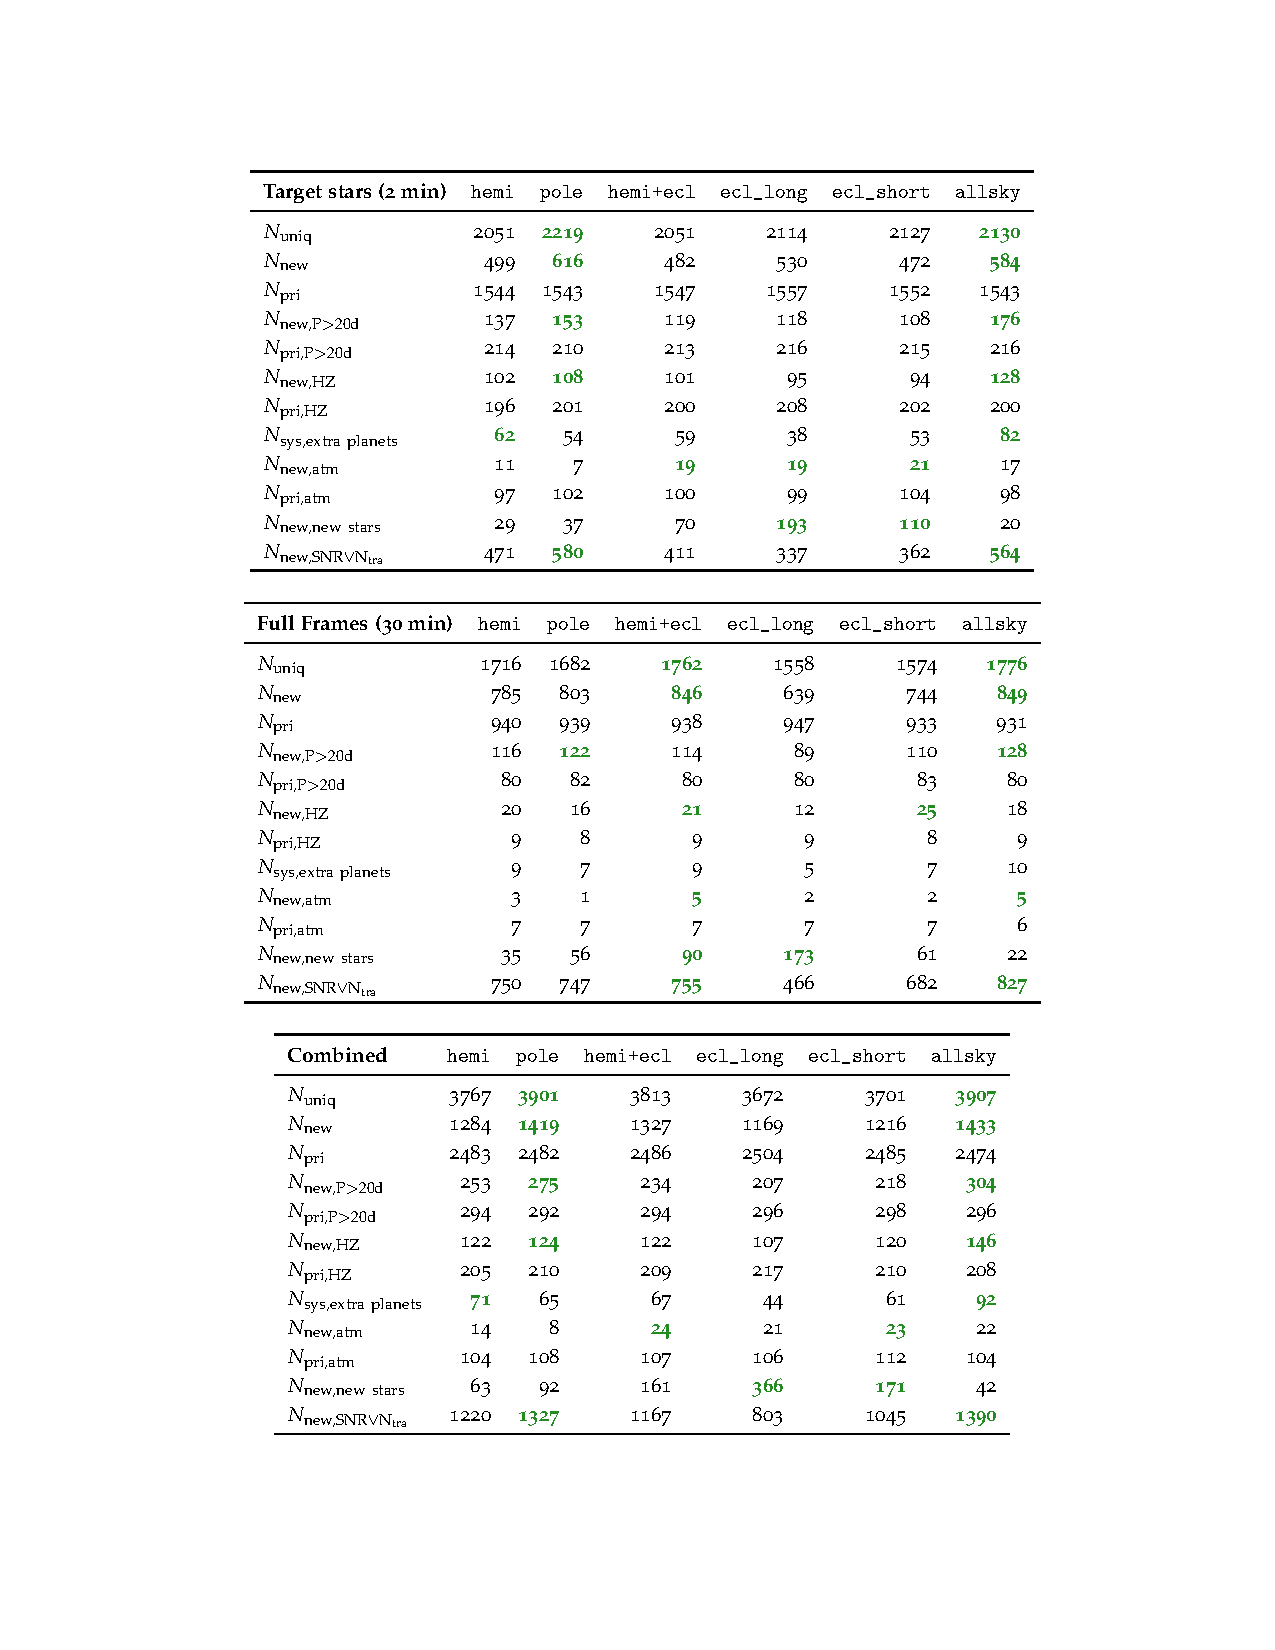
\includegraphics[scale=2.]{tables/cropped_tables_vis.pdf}
	%from 160729_t50 data. generate with tables_vis.tex
	\caption{Detected planet metrics for six possible Extended Missions (values are means of 50 Monte Carlo realizations of our calculation, all for $R_p<4R_\oplus$).
	\textit{Top:} postage stamp detections, \textit{Middle:} full frame image only detections, \textit{Bottom:} sum of both.
	The best two scenarios for select statistics are bolded and highlighted in 
	green.
	\newline
	$N_\mathrm{uniq}$: number of unique planets detected over all 3 years.
	$N_\mathrm{new}$: number of planets detected in year 3 that were not detected in years 1\&2 (newly detected planets).
	$N_\mathrm{pri}$: number of planets detected in the Primary Mission (years 1\&2).
	$N_\mathrm{new,P>20d}$: number of newly detected planets with orbital periods greater than 20 days.
	$N_\mathrm{pri,P>20d}$: same as previous, but from the Primary Mission.
	$N_\mathrm{new,HZ}$: number of newly detected planets satisfying $0.2<S/S_\oplus<2.0$ (approximate habitable zone).
	$N_\mathrm{pri,HZ}$: same as previous, from the Primary Mission.
	$N_\mathrm{sys,extra\ planets}$: number of systems in which extra planets are detected.
	$N_\mathrm{new,atm}$: number of newly detected planets with SNR in transmission greater than (that of GJ 1214b)/2, as measured by \jwst\,-- see text.
	$N_\mathrm{pri,atm}$: same as previous, from Primary Mission.
	$N_\mathrm{new,new\ stars}$: number of newly detected planets that orbit stars that were not observed during the Primary Mission.
	$N_\mathrm{new,SNR\lor N_{tra}}$: number of newly detected planets that were observed during the Primary Mission, but either (a) which had $\mathrm{SNR}<7.3$, a non-detection and/or (b) had $N_\mathrm{tra}<2$, and so would not be `detected'.}
	\label{fig:yield_results}
\end{figure}

For each Year-3 scenario, we compare these numbers to the
corresponding numbers from the Primary Mission as well as to the other
5 scenarios for Year 3. We show the results of our simulations in
Fig.~\ref{fig:yield_results}.  The first point to notice is that for
all but one of the new planet detection metrics ($N_\mathrm{new}$,
$N_\mathrm{new,P>20d}$, $N_\mathrm{new,HZ}$,
$N_\mathrm{sys,extra\ planets}$, $N_\mathrm{new,atm}$,
$N_\mathrm{new,SNR\lor N_{tra}}$) the yields between Extended Missions
vary by less than a factor of two.  The exception is in
$N_\mathrm{new,new\ stars}$, in which \elong\:detects roughly twice as
many planets orbiting never-before-observed stars as any other
proposed mission.

The second point is on the absolute yields of new planets: postage stamp observations find $\mathcal{O}(500)$ new planets, relative to the Primary Mission's $\mathcal{O}(1500)$.
Full frame image observations find $\mathcal{O}(800)$ new planets, relative to the Primary Mission's $\mathcal{O}(900)$.
All Extended Missions find $\mathcal{O}(1300)$ new planets, relative to the Primary Mission's $\mathcal{O}(2500)$.
We discuss these results -- the rough invariance of the number of new planets to different pointing scenarios, and the essential contribution of FFIs -- further in point \#1 below.

Skimming the bottom panel for which missions are highlighted in green when accounting for both PSs and FFIs, we see that \npole\:and \hemis\:are the `superlative-winning' missions in terms of detected planet statistics: considering both PSs and FFIs, \npole\:places top-2 in 5 of 8 relevant categories, and \hemis\:does the same in 6 of 8.
They both do well at maximizing the number of newly detected planets, while also performing well at detecting long period planets, and thus planets in their stars' habitable zones.
\hemis\:also has the largest number of systems in which extra planets are detected.

We now discuss each metric in more depth:
\begin{enumerate}
	\item $N_\mathrm{new}$: we detect about as many new planets in Year 3 as we detect planets in either Years 1 or 2: roughly $1250$.
	The worst and the best scenarios (\elong\:and \hemis, respectively) differ only by a factor of 1.2.
	The fact that there are so many new planets to be detected from extended observations, particularly from full frame images, and that the absolute number of new planets is roughly invariant to the spacecraft's pointing, can be understood from Fig.~\ref{fig:snrf_histogram}.
	This figure illustrates a point that was originally noted by~\citetalias{Sullivan_2015}:
        \tesss Primary Mission will miss many short-period planets around bright stars, and is therefore
        incomplete even its intended hunting ground.
        For stars with $I_c>9$, there are at least an order of magnitude more $R_p<4R_\oplus$ transiting planets that \tess does not detect (Fig 22 of~\citetalias{Sullivan_2015}).
	Our findings agree: there are a substantial number of planets just below the detection threshold, predominantly with $2R_\oplus < R_p <4R_\oplus$ (Fig.~\ref{fig:primary_planet_yield}).
	An Extended Mission will probe and detect this population, irrespective of where on the sky we observe.
	This result should hold equally well for realistic detection efficiency thresholds, and it demonstrates that extended observations will be valuable, because \tess will not yet be at the point of diminishing returns for longer observations (which will happen when more observations only allow pushing out to longer orbital periods). 
	There will still be small, short-period candidates to discover after \tesss Primary Mission.
\begin{figure}[!t]
	\centering
	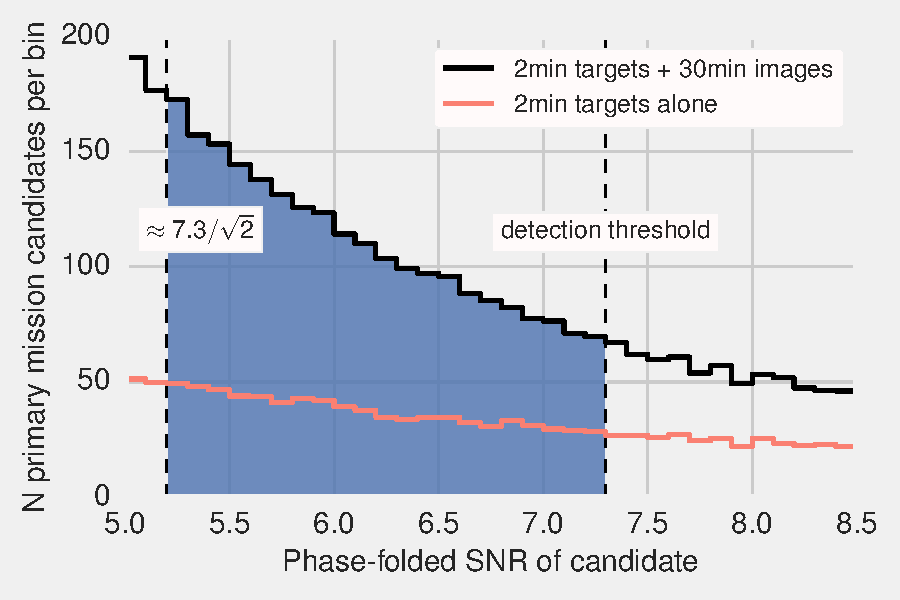
\includegraphics[scale=1.]{figures/snrf_histogram_with_ps.pdf}
	\caption{Histogram of phase-folded SNRs for candidate $R_p<4R_\oplus$ planets following the Primary Mission (from both PS and FFI observations; values are means of 20 Monte Carlo trials; $N_\mathrm{tra}\geq2$).
	If an Extended Mission observes half of the sky, it roughly doubles the number of observed transits for half of the planets observed in the Primary Mission, enabling detection of $\approx 2316/2 = 1158$ planets (half of the blue integrated area in the plot). This coarse estimate is a similar result to our detailed calculations, and shows the value of continuing \tesss observations \textit{irrespective of where we observe}.}
	\label{fig:snrf_histogram}
\end{figure}

	\item $N_\mathrm{new,P>20d}$: it will be possible to detect as many new $P>20$ day planets in one year of \tesss Extended Mission as in both years of the Primary Mission.
	The Primary Mission detects about 295 such planets; \hemis\:and \npole\:scenarios detect similar amounts.
	These two scenarios are achieving the goal of long-period planet detection in slightly different ways: % (see discussion in Sec.~\ref{sec:discussion}):
	\npole\:maximizes the average observing baseline per star, while \hemis\:observes the greatest possible number of stars for longer than 40 days.
	The latter approach could succeed at detecting many planets (our result is that \hemis\:detects the most $P>20$ day planets), but it relies heavily upon the assumption that we can detect planets from only two transits over the course of the entire mission, even if this means only one transit in the Primary, and one transit in the Extended.

	This point -- that the ability of the \hemis\:scenario to detect many long period planets is grounded on the assumption that two transits at high enough SNR are sufficient for detection -- is made explicit in the right panel of Fig.~\ref{fig:Ntra_hist}.
	About half of the long period planets that \hemis\:finds are detected with only two transits.
	By way of comparison, \npole\:detects most of its long-period planets with $\ge 4$ transits.
	This means that the \npole\:detections are more secure.
	For two-transit detections, especially those separated by a gap of a year or more in the \tess data, it will be
        difficult to be confident in either the detection or in the derived 
        orbital period.
        Experience from the \kepler mission showed that requiring 3 or more self-consistent transits substantially lowers the fraction of false signals~\citep{burke_Q1Q8_2014}.
	In cases with a relatively high SNR per transit it is possible to confirm candidates, but with less certainty than if we had more transits in the first place.
	\begin{figure*}[!t]
		\centering
		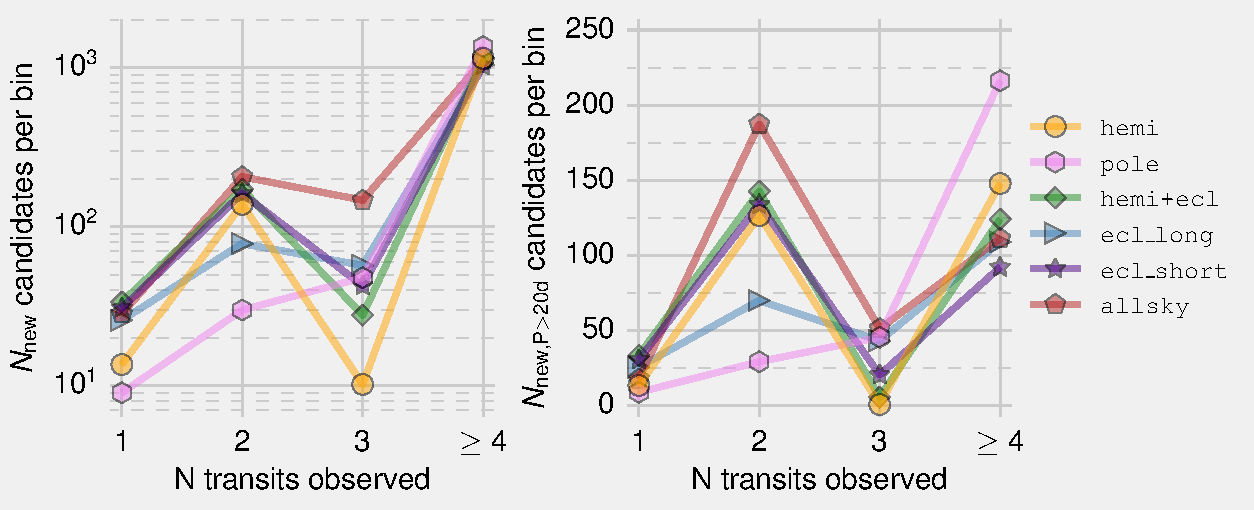
\includegraphics[scale=1.]{figures/Ntra_histogram.pdf}
		%this figure uses 160802 data, which should be the same as 160728_t50, but has ntra_min set to 1 in yieldCode. Read my notes from ext_sim_notes on this -- something's a bit off with the normalization. That said, rather than redo the previous figures with a code that might have a minor bug, my point here -- which is the hemis14d has this issue with few-transit detections -- isn't really any different.
		\caption{ \textit{Left:} Histogram of new $R_p<4R_\oplus$ planet candidates from each Extended Mission as a function of the number of observed transits.
		Candidates are `detected' in Fig.~\protect\ref{fig:yield_results} if $N_\mathrm{tra}\geq2$.
		\textit{Right:} Same as left, restricted to $P>20$ day planets.
		If any given scenario has a `bump' at 2 observed transits, then that scenario depends more heavily on our assumption of being able to make detections based on only two transits.
		Lines between points have no physical meaning; they are intended to improve readability.}
		\label{fig:Ntra_hist}
	\end{figure*}
	\begin{marginfigure}[3in]
		\centering
		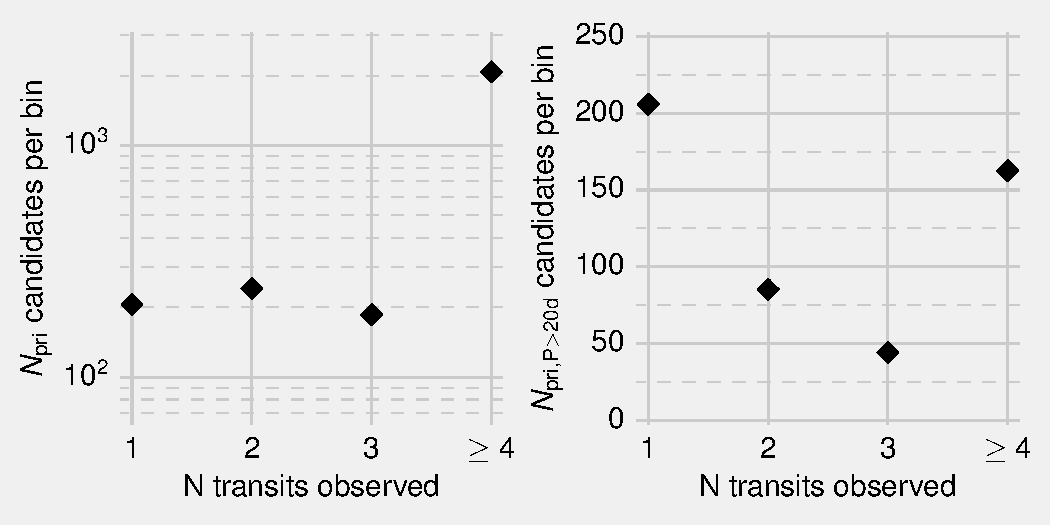
\includegraphics[scale=1.]{figures/Ntra_histogram_primary.pdf}
		%\missingfigure{histogram of Primary Mission number of transits for detected planets}
		% this figure uses BLAH data
		\caption{ 
			Similar to Fig.~\protect\ref{fig:Ntra_hist}, but for the Primary Mission.
		}
		\label{fig:Ntra_hist_primary}
	\end{marginfigure}
	\item $N_\mathrm{new,HZ}$: we approximate the habitable zone as the geometric shell around a host star in which a planet's insolation satisfies $0.2>S/S_\oplus>2.0$.
	With this approximation, the \hemis\:scenario finds the most new habitable zone planets: 146 (which is subject to the same caveats discussed above for long period planet detections). 
	The next-best scenarios, \npole, \npole\:and \shemiAvoid, all detect around 120.
	Relative to the Primary Mission's 210 detections, this means Extended Missions boost the number of detected habitable zone planets by a factor of $\sim1.6$.
	For purposes of weighing the value of habitable-zone detections in deciding between missions, the result that these scenarios all detect a similar number of planets indicates that this metric will likely not `tip the scales' in any direction.
	
	We note in passing that $\sim\!80\%$ of the habitable zone planets that \tess detects orbit M dwarfs with spectral classes ranging from M4 - M0, and $\sim\!15\%$ of them orbit M dwarfs later than M4.
	We show the relevant cumulative distribution in Fig.~\ref{fig:CDF_habitable_zone}.
	% see hz_primary_george/CDF_most_HZ_planets_orbit_early_M_dwarfs.png
	Additionally, our values for the number of $0.2<S/S_\oplus<2$ planets from the Primary Mission are slightly revised from those of~\citetalias{Sullivan_2015}: while~\citetalias{Sullivan_2015} found $48\pm7$ planets with $0.2<S/S_\oplus<2$ and $R_p<2R_\oplus$, we find $34 \pm 5$ such planets.
	Adopting the habitable zone of~\citet{kopparapu_habitable_2013},~\citetalias{Sullivan_2015} found $14\pm4$ planets with $R_p<2R_\oplus$. We find $11 \pm 3$ such planets.
	The rule of thumb that Extended Missions give roughly $1.6\times$ the number of new $0.2<S/S_\oplus<2$ habitable zone planets applies to the~\citet{kopparapu_habitable_2013} habitable zone as well as $0.2<S/S_\oplus<2.0$.
	Another point raised by Fig.~\ref{fig:scatter_habitable_zone} is that the~\citet{kopparapu_habitable_2013} habitable zone, which is physically motivated by 1-D radiative-convective cloud-free climate models with accurate absorption coefficients, results in roughly 3 times fewer `habitable zone' planet detections than our ad-hoc criterion of $0.2<S/S_\oplus<2$.
	\begin{marginfigure}
		\centering
		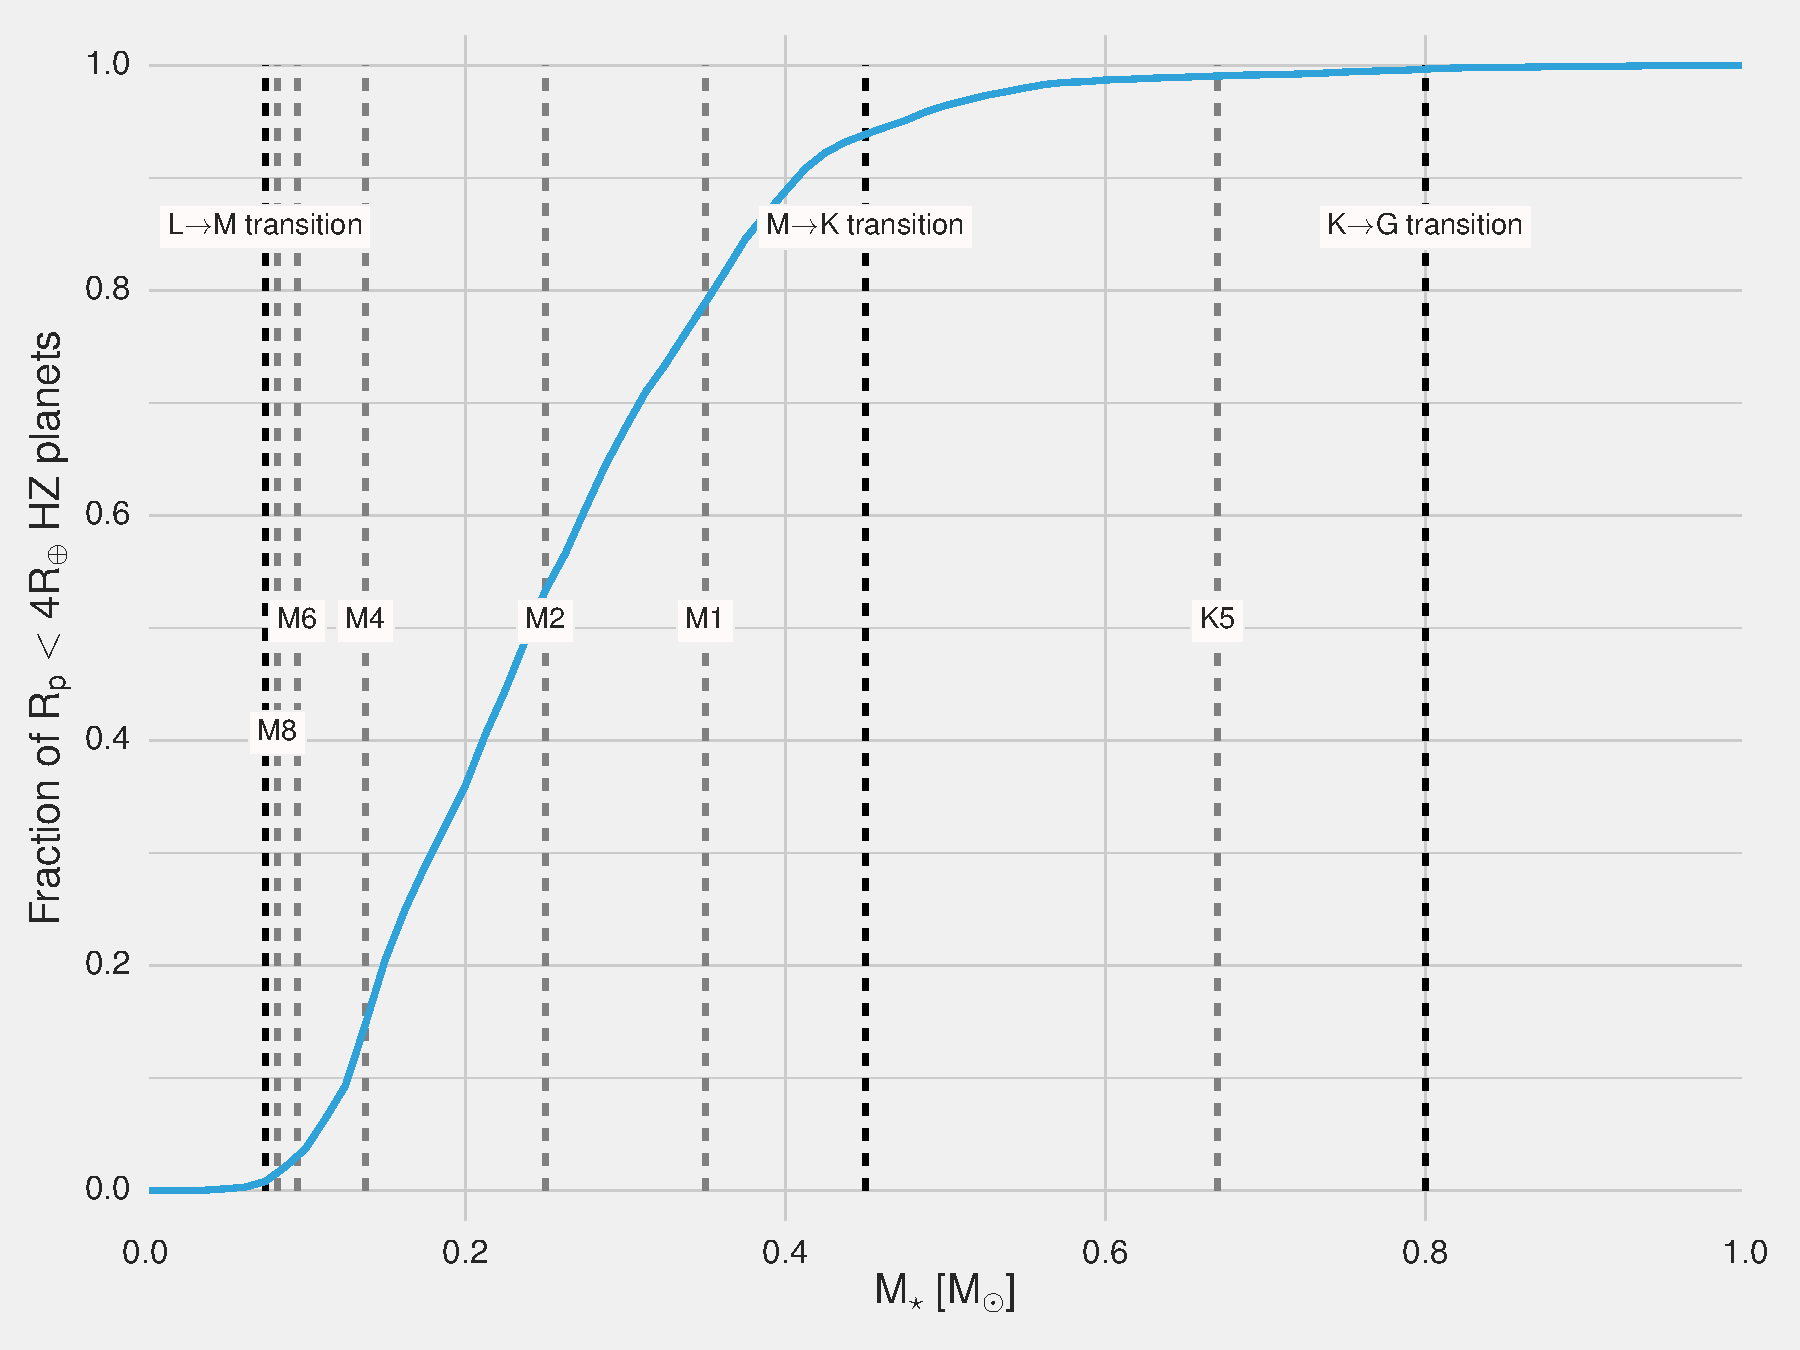
\includegraphics[scale=1.]{figures/CDF_most_HZ_planets_orbit_early_M_dwarfs.pdf}
		\caption{Cumulative distribution of $R_p<4R_\oplus$ and $0.2<S/S_\oplus<2$ planet candidates from the Primary Mission (a proxy for the habitable zone). Boundaries of spectral classes are highly approximate, and taken from from~\protect\citet{habets_empirical_1981} and~\protect\citet{baraffe_massspectral_1996}.}
		\label{fig:CDF_habitable_zone}
	\end{marginfigure}
	\begin{marginfigure}
		\centering
		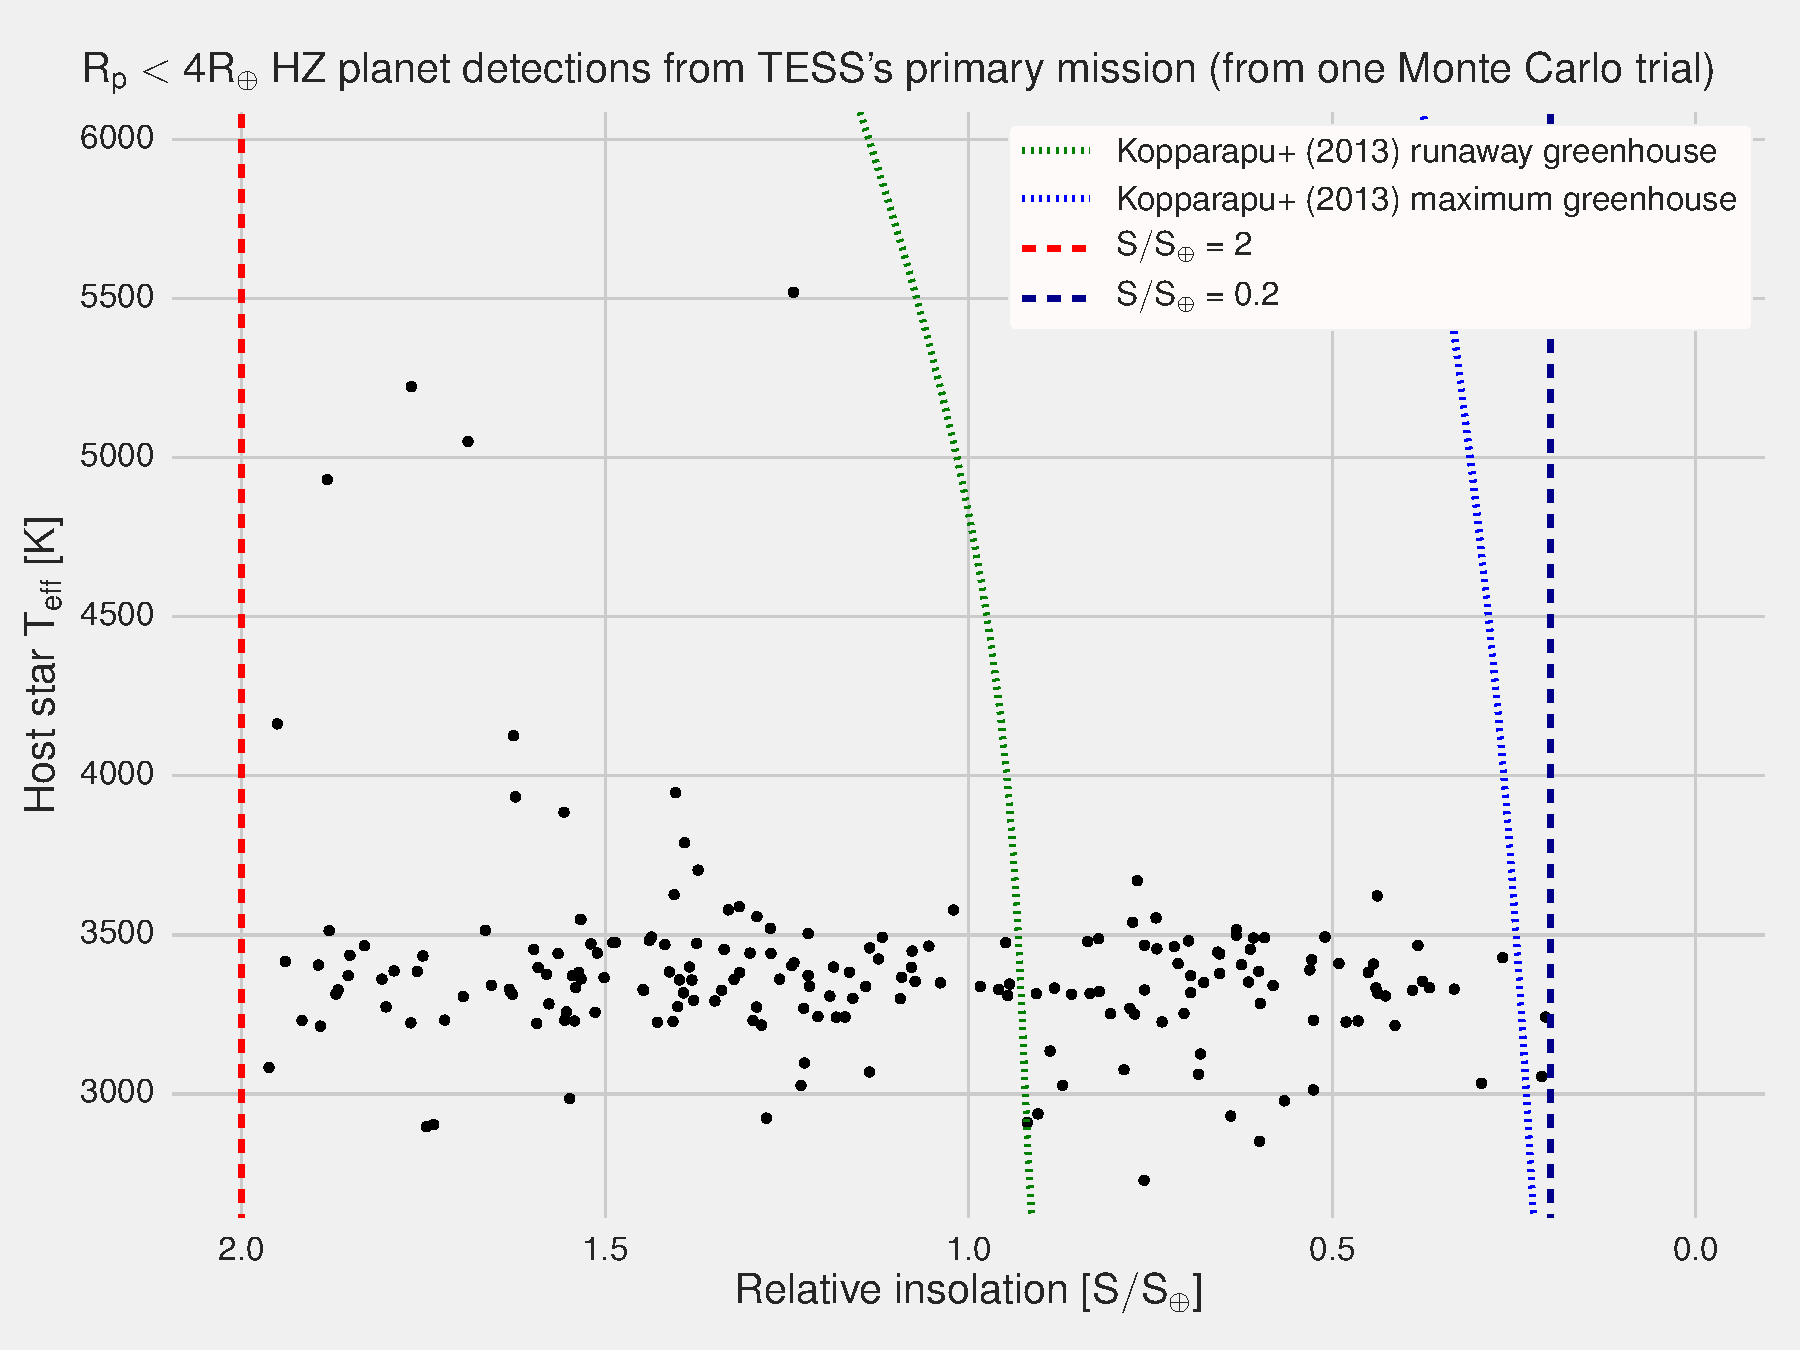
\includegraphics[scale=1.]{figures/hz_planet_detections_rp_lt_4re_kopparapu_2013_incl.pdf}
		\caption{Scatter plot of $R_p<4R_\oplus$ planet candidates falling in the~\protect\citetalias{Sullivan_2015} or \protect\citet{kopparapu_habitable_2013} habitable zones. }
		\label{fig:scatter_habitable_zone}
	\end{marginfigure}	
	
	\item $N_\mathrm{sys,extra\ planets}$: for how many systems do we detect extra planets?
	Our assumptions about multiple planet system distributions are crude -- we assume independent probability draws from single planet occurrence distributions.
	Thus our simulated planet population does not have systems of tightly packed inner planets in realistic numbers.
	That said, we expect this statistic to be some indication of the information that we are not explicitly modeling, but which can be obtained from extended observations of planetary systems post-planet detection. 
	This additional information includes improved precision on physical and dynamical parameters of the system.
	It also includes transit timing variations, which could be used to discover non-transiting planets as well as transiting outer companions.
	TTVs can also give dynamical hints for the formation history of planetary systems, for instance, discriminating between \textit{in situ} formation and inward migration as~\citet{mills_resonant_2016} argued for the Kepler 223 system.
	
	The most prominent feature in the results for this metric is that \elong\:detects the fewest systems with extra planets (44, which is $39\%$ worse than the next-best). 
	This is reasonable because \elong\:spends the most time looking at new sky, and in the process observes fewer systems that were detected in the Primary Mission.
	\nhemi, \shemiAvoid, \npole, and \eshort\:all perform similarly, detecting $\sim65$ such planets.
	\hemis\:detects the most, at 92. While this is still subject to the assumption of two-transit recoverability, in this case the requirement is not too strong: only 10 of \hemis's systems with newly detected planets come from the case where the extra detected planet comes from two transits.
	% makeReport: search for "ntrahemis14d". same for commit.
	
	\item $N_\mathrm{new,atm}$:
	  We define `planets that are amenable to atmospheric characterization' to mean planets whose SNR in transmission is at least half as large as that of GJ~1214b. We chose ``at least half as large'' rather than
          ``equal to'' in order to give a sufficiently large sample to prevent Poisson fluctuations from hindering our comparisons.
	The relevant signal in transit spectroscopy is the ratio of the areas of atmosphere's annulus to the star's disk on the sky plane, $\delta_\mathrm{atm} = 2\pi R_p h_\mathrm{eff}/(\pi R_\star^2)$, where the effective scale height of the atmosphere $h_\mathrm{eff}$ is proportional to the actual scale height.
	Assuming that the planet is in thermal equilibrium with incident radiation from the host star, and that its atmosphere has known mean molecular weight and Bond albedo, we can compute a representative signal.
	The noise performance depends on the observing instrument, and could be complex if not simply dominated by shot-noise from IR photons.
	We circumvent such complexities via an empirical formula provided to us by Drake Deming, based on a multi-variate regression fit to detailed simulations performed by Dana Louie.
	This formula estimates the SNR in transmission from 4 transits observed with \jwsts NIRISS instrument:
	\begin{align*}
	\log_{10} \mathrm{SNR} =\ &2.98\log_{10}\left(\frac{R_p}{R_\oplus}\right)
							 - 1.019\log_{10}\left(\frac{M_p}{M_\oplus}\right) \\
							 &- 1.459\log_{10}\left(\frac{R_\star}{R_\odot}\right)
							 - 0.249\log_{10}\left(\frac{a}{\mathrm{AU}}\right) \\
							 &- 0.147\left(V - 5.0\right) + 0.193  \numberthis
	\label{eq:atmosphere_Deming}
	\end{align*}
	for $V$ the host star's apparent $V$-band magnitude (calibrated for $3>V>22$), $R_p$ the planet radius, $M_p$ the planet mass, $R_\star$ the star radius, and $a$ the planet's semi-major axis.
	The coefficients are physically sensible: the 2.98 coefficient of $R_p$ minus the 1.019 coefficient of $M_p$ implies that the SNR depends inversely as bulk density, with puffier planets giving higher SNR for transit spectroscopy.
	Although this formula uses a $V$ band magnitude ($\approx$0.5--0.6$\mu$m), while NIRISS's SOSS mode covers 0.6--2.8$\mu$m, the only difference if we were to use $J$ band magnitudes would be in the coefficients preceding the stellar radius and the semi-major axis terms (and thus implicitly, in the stellar mass).
	Focusing our analysis to a SNR measured by \jwst is sensible given \tesss role as a `\jwst finder scope'~\citep{deming_jwst_tess_2009}.
	We focus specifically on NIRISS given that it will likely be the workhorse \jwst instrument for transmission spectroscopy~\citep{beichman_observations_2014}.
	\begin{figure*}[!th]
		\centering
		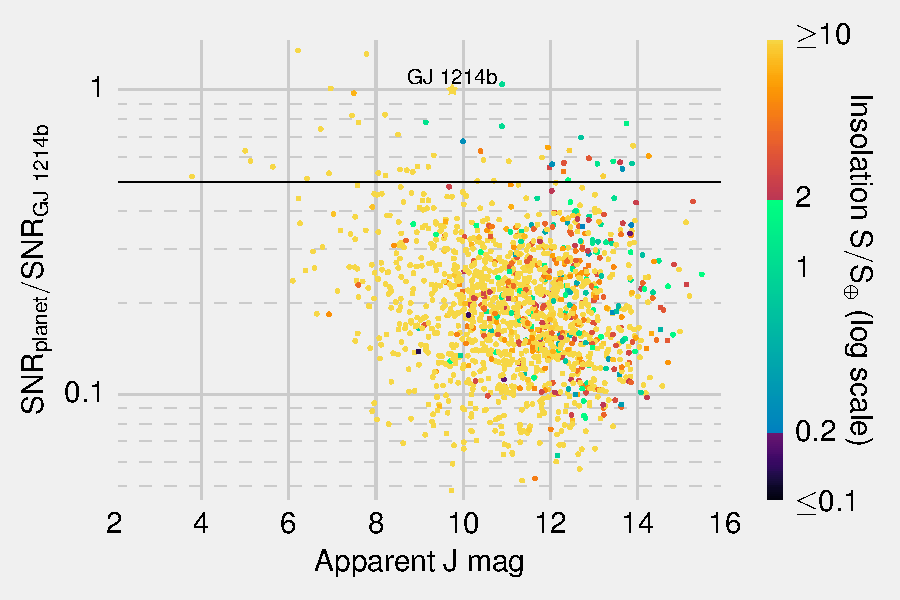
\includegraphics[]{figures/SNR_in_transmission.pdf}
		\caption{ Scatter plot showing the SNR in transmission of detected planets with $R_p<4R_\oplus$ from one Monte Carlo realization of all 3 years of the \npole\:scenario.
			The SNR is computed from Eq.~\protect\ref{eq:atmosphere_Deming}.
			Planets above the horizontal black line ($\mathrm{SNR_{planet}/SNR_{GJ\ 1214b}} = 0.5$) are counted for Fig.~\protect\ref{fig:yield_results}'s metric of planets with `good' atmospheres for transmission spectroscopy.
			GJ 1214b is marked with a star.
			The coloring of planets indicates their relative insolation, as well as whether they fall our ad-hoc habitable zone ($0.2<S/S_\oplus<2)$.
		}
		\label{fig:atmosphere_scatter}
	\end{figure*}

	The system values for GJ 1214b are those found
	by~\citet{charbonneau_gj1214b_2009}: $R_p = 2.678R_\oplus$, $M_p = 6.55M_\oplus$,
	$R_\star = 0.211R_\odot$, $a = 0.0144\mathrm{AU}$, $V = 15.1$.
	Using Eq.~\ref{eq:atmosphere_Deming}, we compute the SNR in transmission for all detected planets, for all Extended Mission scenarios.
	Fig.~\ref{fig:atmosphere_scatter} shows one realization of the resulting distribution for planets detected in all three years of the \npole\:scenario.

	\tess mostly detects strongly irradiated planets (most points on Fig.~\ref{fig:atmosphere_scatter} are yellow).
	A very small number, $\lesssim 10$, are both in the approximate habitable zone and also `favorable for atmospheric characterization'.
	Of course, a highly compelling target with lower SNR in transmission per transit might merit a more ambitious \jwst observing program.
	We note that all of these planets are assumed to have identical mean molecular weights and cloud properties.
	%\todo[inline]{what cloud model/opacity does this use?}

	More importantly, Fig.~\ref{fig:yield_results} shows that most of the planets with atmospheres that are best for transmission spectroscopy are already discovered after two years.
	The best Extended Missions (\shemiAvoid, \elong, \eshort\:and \hemis) boost the yield of such planets from $\sim\!100$ to $\sim\!125$.
	The worst, \npole, finds about an additional 10.
	This best-case boost of $1.25\times$ more `good' planets for atmospheric characterization is less than the relative boost of $1.6\times$ more newly detected long period planets.
	Put differently, among the various possibilities for the Extended Mission,
        there is more variation in $N_\mathrm{new,P<20d}$ than in $N_\mathrm{new,atm}$.
	
	
	\item $N_\mathrm{new,new\ stars}$:
	  Intuitively we expect that to maximize the number of planets detected 
	  around ``new'' stars (those which were not observed during the Primary 
	  Mission) we should collect as many photons as possible from new stars.
         And the region on the sky with the greatest number of new stars is the ecliptic.
	 It is not surprising, then, that the \elong\:scenario finds the largest number of planets around new stars.
         The \elong\:scenario dedicates 7 of a single year's 13 observing sectors to the ecliptic (where the other 6 are spent centered at the North Ecliptic Pole due to excessive Earth and Moon crossings).
	It consequently detects twice as many new planets about newly observed stars as the next-best scenarios: \eshort\:and \shemiAvoid\:(366 vs 171 and 161, respectively).
	These latter two scenarios also spend time observing the ecliptic, but with 
	only one camera, rather than with all four cameras simultaneously.
	We note that even though \elong\:is the scenario most successful in detecting planets about new stars, the new stars represent only $\sim\!30\%$ of the total number of new detections.~\footnote{Here, we remind the reader that ``new'' refers only to \tess observations. Some of these stars will
          have been observed by K2 or other projects (see discussion in Sec.~\ref{sec:discussion}).}

	\item $N_\mathrm{new,SNR\lor N_{tra}}$:
	This statistic is the number of newly detected planets that are detected either (a) due to their final SNR clearing our threshold (logical) or (b) their number of observed transits being greater than or equal to 2.
	It is the complement to $N_\mathrm{new,new\ stars}$: scenarios like \nhemi, \npole, and \hemis\:that do not observe many new stars will detect all of their planets from a boosted SNR and/or clearing the minimum transit threshold.
	
\end{enumerate}

\paragraph{Comment on meaning of `detected in postage stamps' vs `detected in FFIs'}
The invested reader may inquire ``what about the cross-over case of planets that are observed as PSs during the Primary (Extended) Mission, but as FFIs in the Extended (Primary) Mission? These are not explicitly listed in Fig.~\ref{fig:yield_results}''.
%This is what is done in Fig.~\ref{fig:yield_results}.
When describing the entire unique planet population detected from Years 1-3, for simplicity of language we use `postage stamp detections' to refer to planets that are observed at any time (Primary or Extended Missions) at 2 minute cadence.
In these cases, the dominant contribution to the final signal to noise ratio tends to come from the PS observations.
When describing new planet detections, we use `postage stamp detections' to mean planets that were newly detected due to being observed as postage stamps in the Extended Mission.
In other words, this `cross-over' point only matters in discussions of the unique planet population from an entire mission, Years 1-3.
Considering just the newly detected planet population, we can unambiguously specify whether the new detections came from full frame images or postage stamps, irrespective of their observations from the Primary Mission.


\subsection{On the Brightness of Stars with Detected Planets}
\begin{figure}[!t]
	\centering
	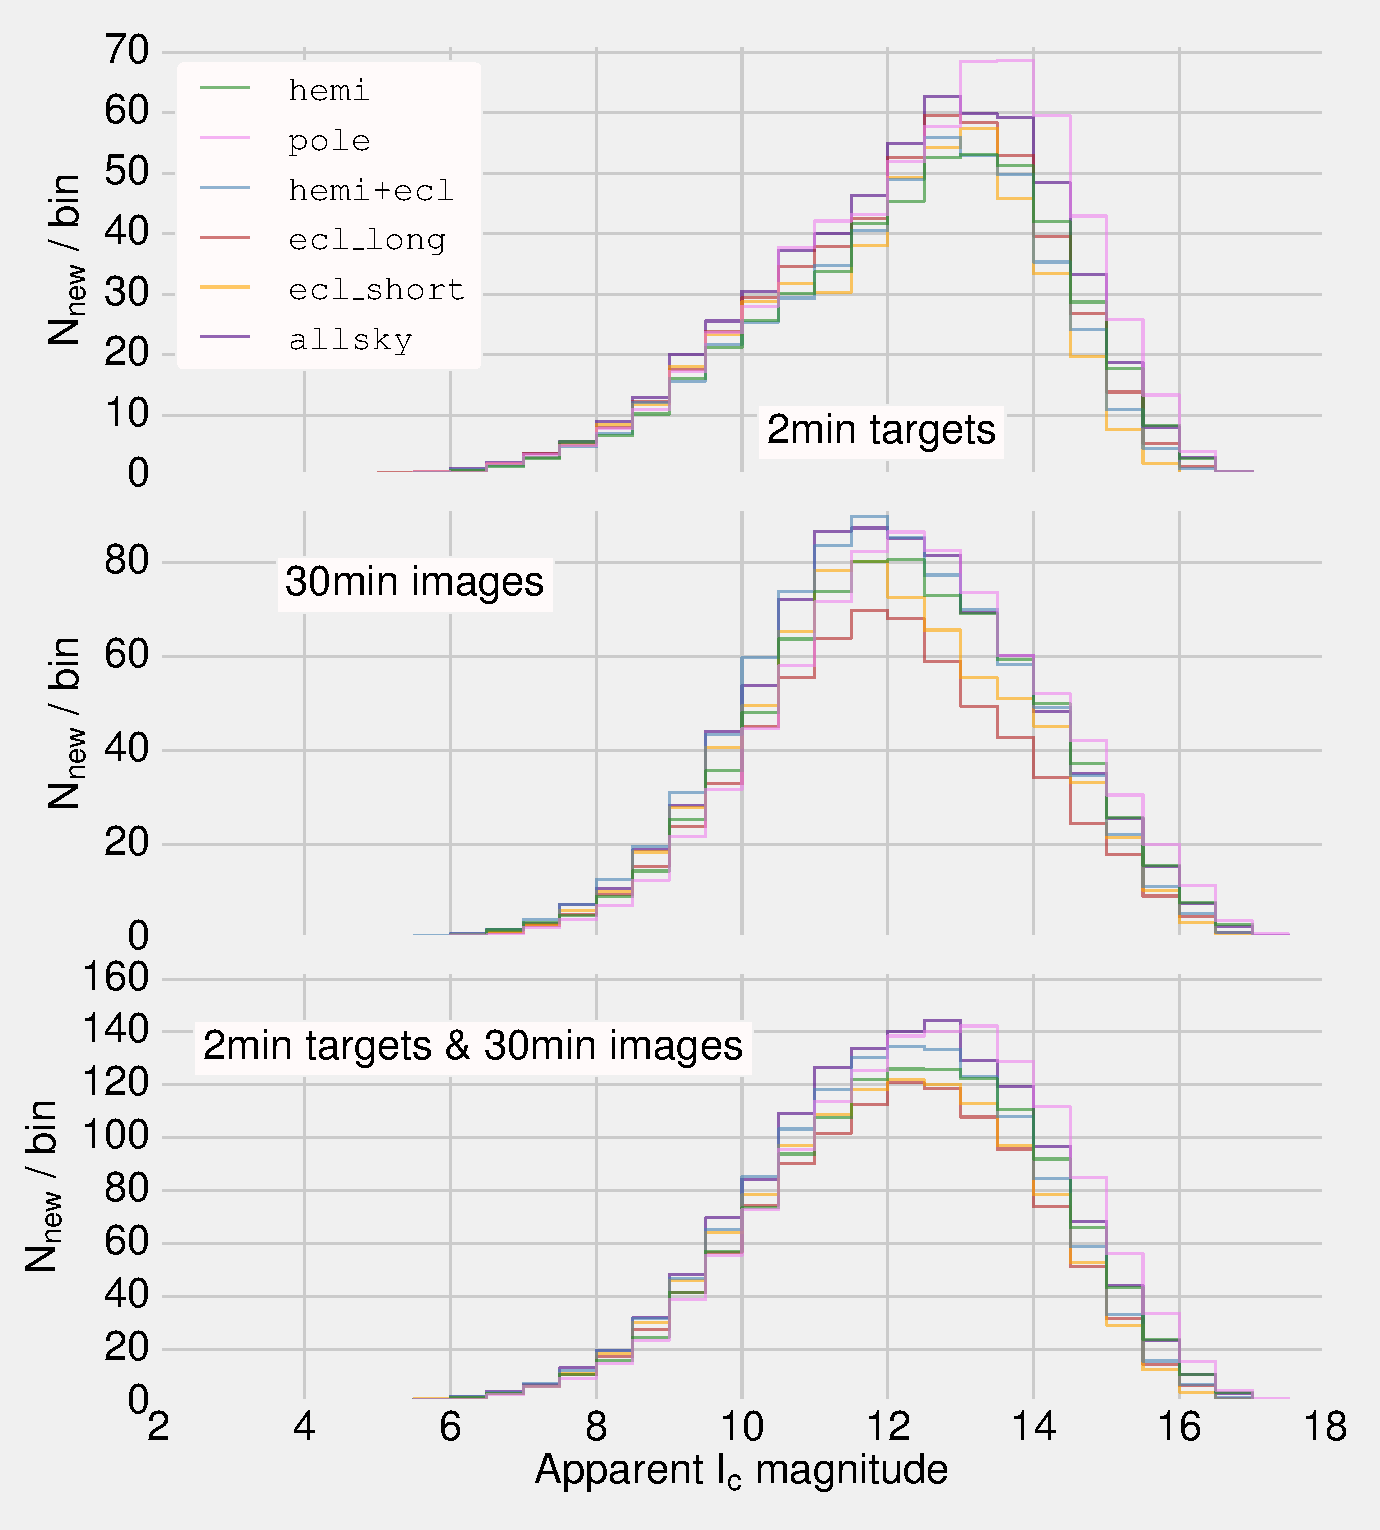
\includegraphics[]{figures/160729_icmag_t50_all.pdf}
	\caption{Histogram of apparent $I_c$ magnitude of host star for newly detected $R_p<4R_\oplus$ planets from all Extended Mission scenarios, for \textit{top:} postage stamp detections, \textit{middle:} full frame image detections, \textit{bottom:} the sums thereof.
	While \npole\:does well by most metrics, a larger proportion of the new planets it detects orbit dim stars compared to alternatives like \hemis\:or \shemiAvoid.}
	\label{fig:icmag_meta}
\end{figure}
While \npole\:does well by most metrics, a larger proportion of its newly 
detected planets orbit dimmer stars than the planet populations detected from 
alternatives like \hemis\:or \shemiAvoid.
We demonstrate this in Fig.~\ref{fig:icmag_meta}.
The main point here is that if our only priority were to maximize the number of new detections around bright host stars, then \npole\:would be the worst among the scenarios considered here.
% then why didn't we include this in fig 13?
For instance, arbitrarily setting the bound at $I_c<10$ and numerically 
integrating from Fig.~\ref{fig:icmag_meta}'s data, we see in 
Table~\ref{tab:icmag_meta} that there is a $\sim30\%$ difference between the 
missions.
For point of reference, the Primary Mission detects 386 such planets -- so a single year of Extended Mission detects roughly as many planets orbiting bright hosts as a single year of Primary Mission.
%cf bright_star_comparison_Ic_lt_10.ipynb
\begin{table}[!ht]
	\centering
	\caption{Number of new, $I_c<10$, $R_p<4R_\oplus$ planets from each Extended Mission (average of 50 Monte Carlo realizations of our code; showing sum of PSs \& FFIs). \npole\:detects the fewest new planets orbiting bright stars.}
	\label{tab:icmag_meta}
	\begin{tabular}{|c|c|c|c|c|c|}
		\hline
		\nhemi & \npole & \shemiAvoid & \elong & \eshort & \hemis \\ \hline
		162    & 154    & 190         & 167    & 183     & 198    \\ \hline
	\end{tabular}
	%I put together this table by running /ext_mission_comparisons/memo_processing with the 160729_t50 data, and then just directly printing the numbers.
\end{table}

\begin{comment}
A related, but minor comment: \tesss is able to detect the smallest planets at the ecliptic poles, rather than near the ecliptic, due to background flux from zodiacal light. 

\begin{figure*}[th]
	\centering
	\todo[inline]{keep this figure? if so, make with 160729 data}
	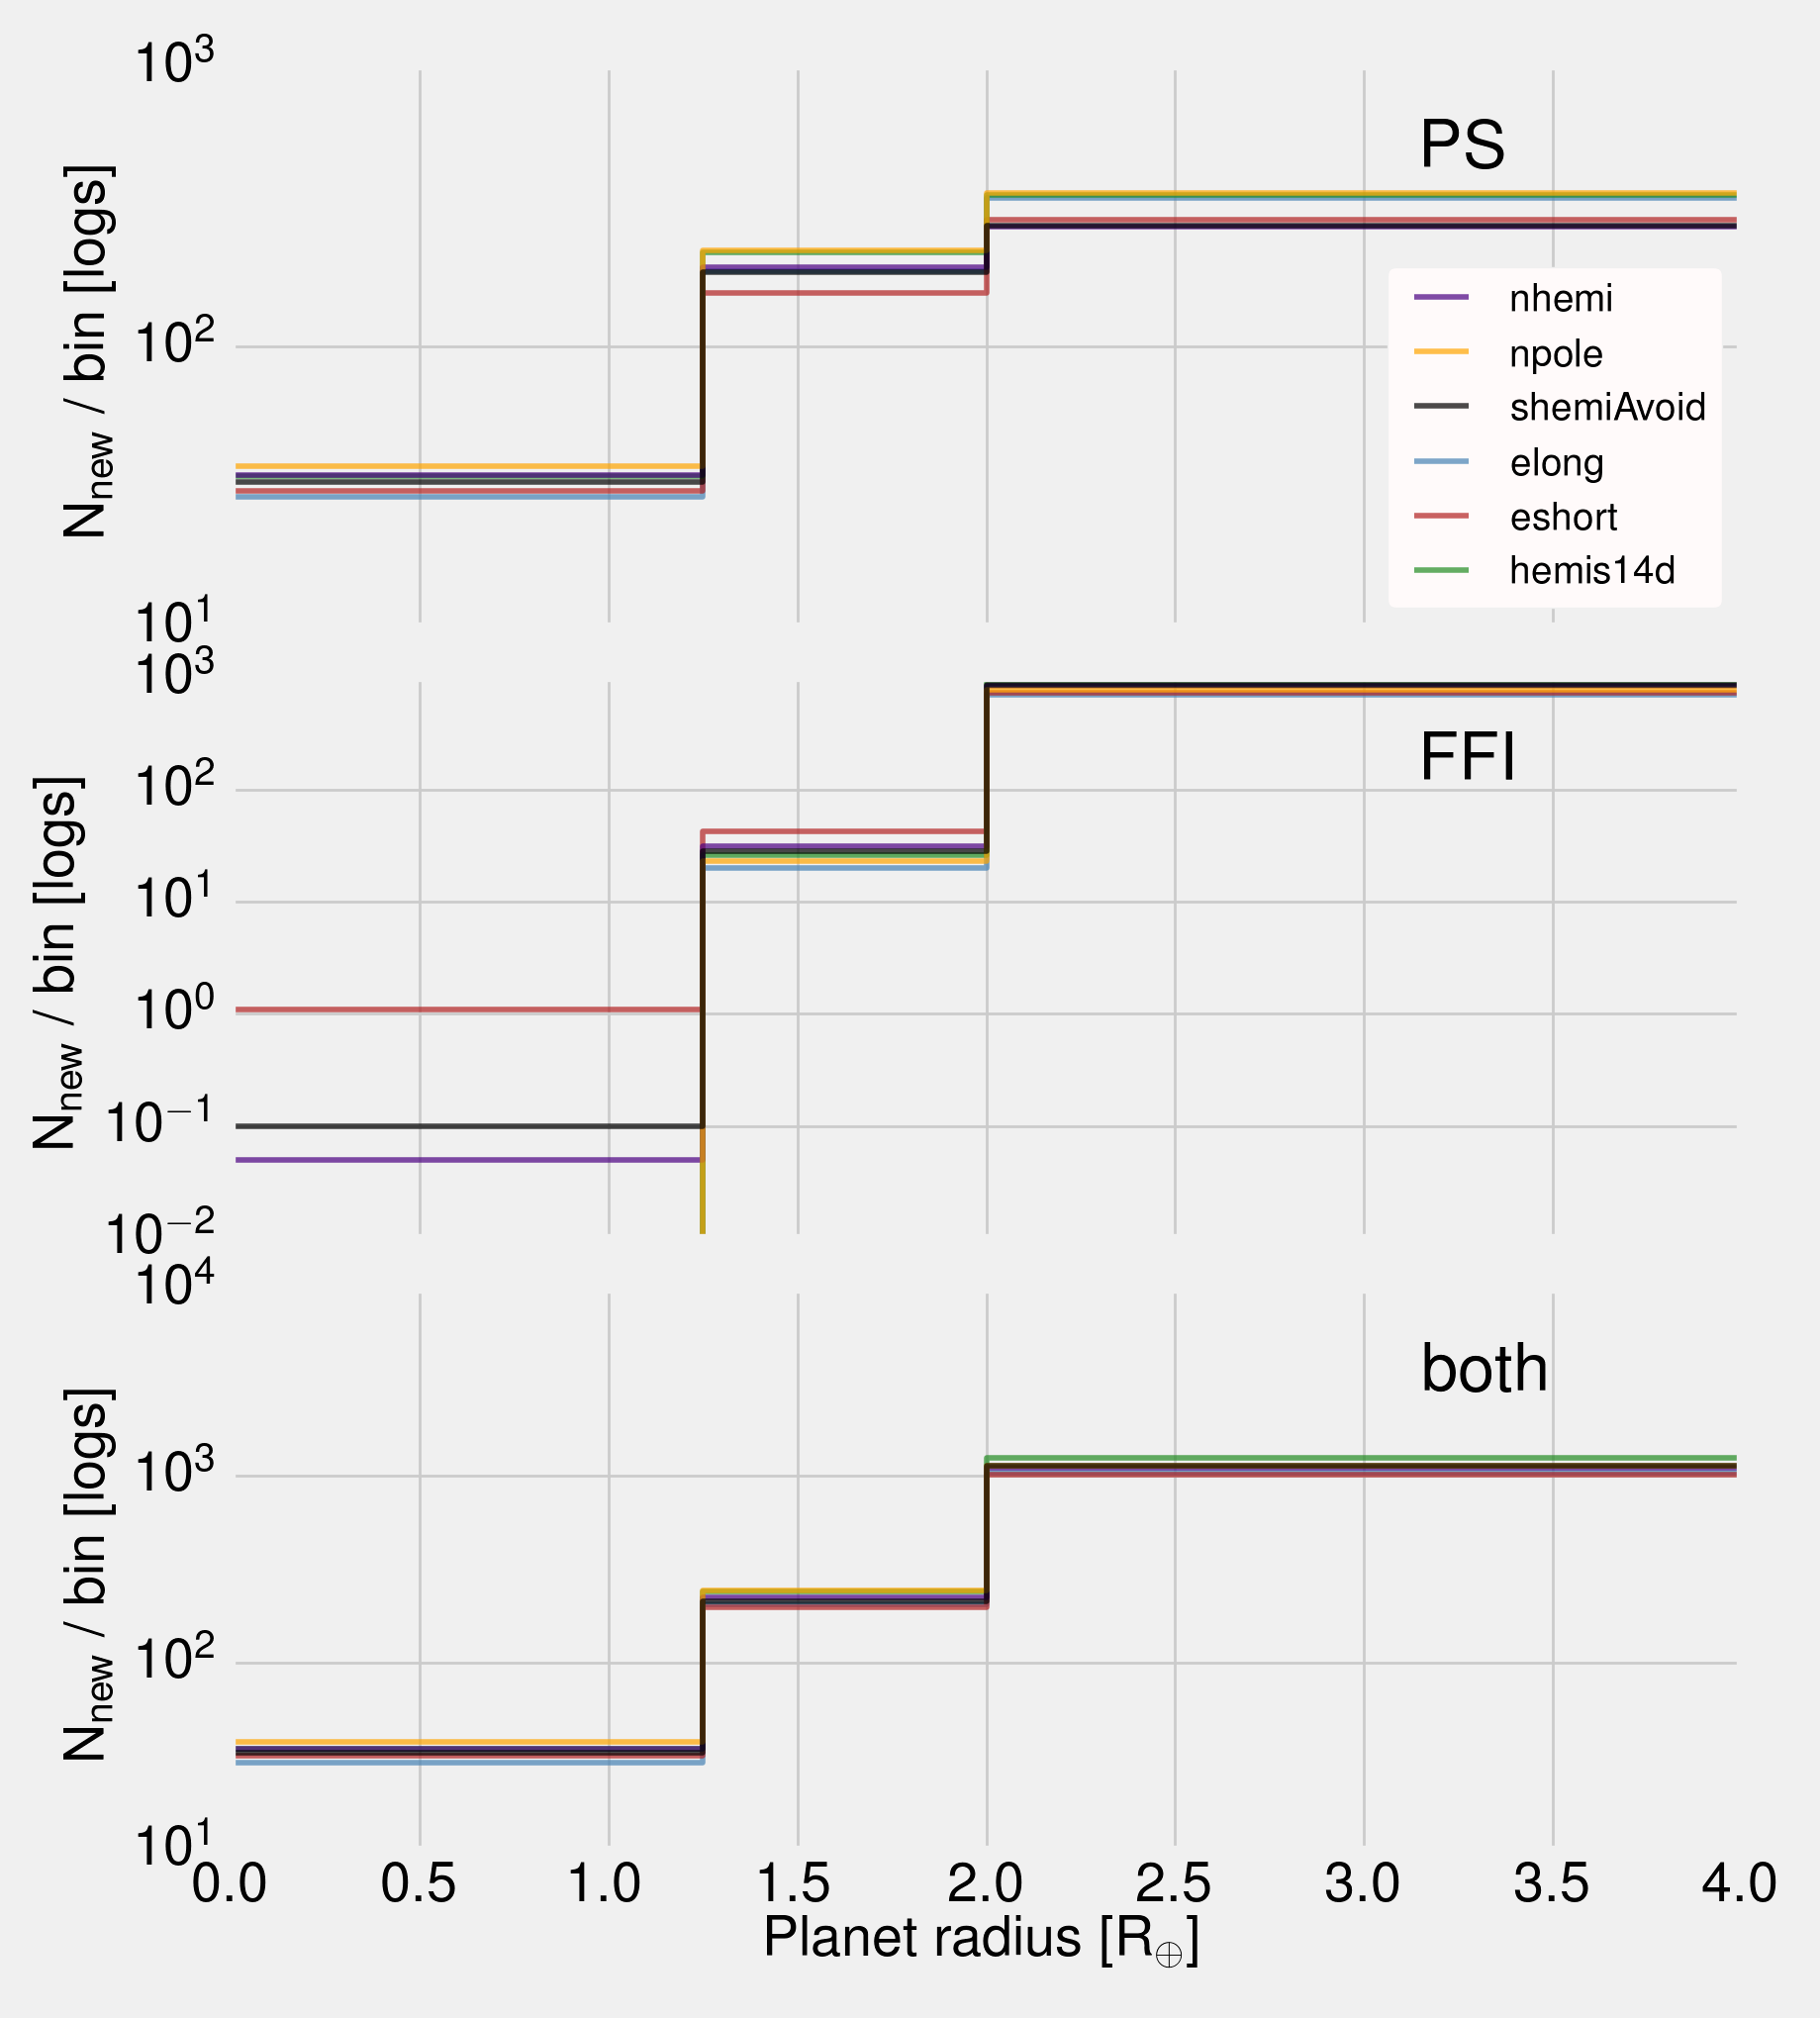
\includegraphics[]{figures/160708_r2_t20_all.png}
	\caption{\textit{Top:} words. \textit{Middle:} words. \textit{Bottom:} words.}
	\label{fig:r2_meta}
\end{figure*}
\end{comment}

